\documentclass[12pt,DIV=15,BCOR=15mm,twoside,headsepline,abstract=true,listof=totoc,bibliography=totoc]{scrreprt}

%%%%%%%%%%%%%%%%%%%%%%%%%%%%%%%%%%%%%%%%%%%%%%%%%%%%%%%%%%%
%%%%%%%%%%%%% Uni Rostock Thesis Style %%%%%%%%%%%%%%%%%%%%
%%% bei Problemen, Mail an susann.dittmer@uni-rostock.de
%%%%%%%%%%%%%%%%%%%%%%%%%%%%%%%%%%%%%%%%%%%%%%%%%%%%%%%%%%%
% enthält schon viele wichtige Pakete
\usepackage[mnf]{thesis_uro} %Fakultät wählen: uni (Standard),inf,msf,ief,mnf,mef,juf,wsf,auf,thf,phf
\usepackage{algorithm}
%\usepackage{algorithmic}
\usepackage{algpseudocode}
\addbibresource{literatur.bib} %Bibliographiedateien laden

%Definition von Umgebungen
\newtheorem{kor}{Korollar}
\newtheorem{hsatz}{Hilfssatz}
\newtheorem{satz}{Satz}
\newtheorem{prop}{Proposition}
\newtheorem{defi}{Definition}
\newtheorem{lem}{Lemma}
\newtheorem{annahme}{Annahme}
\newtheorem{problem}{Problem}
\theoremstyle{remark}	%Styleänderung (Text aufrecht, ...)
\newtheorem{bem}{Bemerkung}
\newtheorem{bsp}{Beispiel}

%Beispiel für eigene Kommandos
\newcommand{\ol}{\overline} %Kurzform für \overline definiert 
%\newcommand{\RR}{\mathbb{R}}
%newcommand{\RRn}{\mathbb{R}^n}

\newcommand{\RR}{\ensuremath{\mathbb{R}}}
\newcommand{\Rnv}{\ensuremath{\mathbb{R}^{n}}}
\newcommand{\Rnn}{\ensuremath{\mathbb{R}^{n\times n}}}

\newcommand{\NN}{\ensuremath{\mathbb{N}}}

\newcommand{\mK}{\ensuremath{\mathcal{K}}}
\newcommand{\mKp}{\ensuremath{\mathcal{K}}^+}
\newcommand{\Code}{\ensuremath{C^{\textnormal{dgl}}}}

% Daten für die Titelseite
\institut{Institut für Mathematik} %auskommentieren, wenn nicht benötigt
\arbeit{Masterarbeit} %Bachelorarbeit, Masterarbeit oder Abschlussarbeit (wenn Staatsexamensarbeit geschrieben wird, kann man, z. B. bei Untertitel "Wissenschaftliche Abschlussarbeit\\ im Rahmen  des Ersten Staatsexamens" eintragen)
\autor{Vorname Nachname}
\betreuerGutachter{Name des Betreuers und ersten Gutachters\newline Universität Rostock\newline Fakultät} %hier \newline als Zeilenwechsel, da Tabelle mit \parbox im Hintergrund
\gutachter{Name des zweiten Gutachters\newline Universität Musterstadt\newline Fakultät}				%dto.
\date{12.08.2021}
\matrNr{123\,45678}
\titel{Titel der Arbeit,\\ bei Bedarf auch zweizeilig}
\untertitel{Untertitel der Arbeit, auch mehrzeilig oder ganz weglassen.} %auskommentieren, wenn nicht benötigt

\begin{document}
\hypersetup{pageanchor=false}
\begin{titlepage}
\mytitle   %hier werden Daten für die Titelseite gesetzt
\end{titlepage}

\zusammenfassung{
  Platz für eine kurze Zusammenfassung.\\
}
\pagenumbering{Roman}
\tableofcontents % Inhaltsverzeichnis
\listoffigures
\listoftables
\addcontentsline{toc}{chapter}{Algorithmenverzeichnis}
\listofalgorithms
\lstlistoflistings

% Abkürzungsverzeichnis --------ggfs auskommentieren
\chapter*{Abkürzungsverzeichnis}
\addcontentsline{toc}{chapter}{Abkürzungsverzeichnis}
\begin{acronym}[SEPSEP]
 \acro{rnn}[RNN]{Rekurrentes Neuronales Netz}
\end{acronym} 


% Symbolverzeichnis ------------ggfs auskommentieren
\chapter*{Symbolverzeichnis}
\addcontentsline{toc}{chapter}{Symbolverzeichnis}
\begin{acronym}[SEPSEP]
 \acro{cm}[$\mathcal{C}$]{Confidence Matrix}
\end{acronym}
\cleardoublepage
\hypersetup{pageanchor=true}
\pagenumbering{arabic}

%mainmatter
\chapter{Einleitung}
!!! eine kurze Einleitung, wird noch verbessert/erweitert, in Kontext CNN einordnen!!!
!!! ist die Einleitung von der Projektarbeit(FeedForwardNetze in SQL)

!!! Literaturnachweise in bibmanager eingügen !!!


Assistenzsysteme stellen Informationen und Hilfestellungen bei bestimmten Produkten bereit, um deren Bedienung zu erleichtern. 
Heutzutage spielen sie in fast allen Bereichen der Industrie und Forschung eine große Rolle und unterstützen Menschen bei ihren Tätigkeiten \cite{winner2014handbook, kurihata2005rainy, omerdic2011design}.
Meist werden solche Systeme intelligent genannt, denn sie sind in der Lage, durch die Verarbeitung von Sensordaten eigenständig auf bestimmte Szenarien zu reagieren beziehungsweise Vorhersagen über zukünftige Situationen zu treffen. Die Analyse solcher Assistenzsysteme ist daher Forschungsgegenstand in den Bereichen der Big Data Analytics und Künstlichen Intelligenz.
Sensoren liefern hierbei im Zusammenhang des \textit{Internet of Things} \cite{xia2012internet, wortmann2015internet} meist große Datenmengen, die geschickt gespeichert und verarbeitet werden sollen. 

Das PArADISE-Projekt \cite{paradise} des Lerhstuhls für Datenbank- und Informationsysteme der Universität Rostock beschäftigt sich mit dem Designsprozess von Assisenzsystemen mit dem Ziel, die Entwickler von assistiven Systemen zu unterstützen. Durch eine hochparallele Analyse großer Mengen von Sensordaten soll hierbei die datengetriebene Entwicklung von Assisenzsystemen gelingen. In der Anwendung werden jene Systeme genutzt, um Vorhersagen über bestimmter Ereignisse durch Algorithmen (Maschinelles Lernen) zu treffen. Verfahren des überwachten maschinellen Lernens lassen sich typischerweise in 2 Schritten durchführen. In einer Trainingsphase werden mit Hilfe von Trainingsdaten per Annotation Modelle zur
Erkennung von Mustern abgeleitet. In der späteren Erkennungsphase wird dann das
trainierte Modell genutzt, um erkannte Muster in einer Zieldatenmenge effizient ableiten
zu können. 

In der Arbeit von Marten \cite{marten2017machine} wird am Beispiel eines Meeting Szenarios ein Maschinelles Lernverfahren namens Hidden-Markov-Modelle untersucht. Es wird erläutert, wie die Erkennungsphase eines zuvor trainierten Modells datenbankgestützt in parallelen SQL-Datenbanksystemen realisiert werden kann.   
Als Ergebnis wird festgehalten, dass die datenbankgestützte Umsetzung von ML-Algorithmen, hier speziell bei Hidden-Markov-Modellen, in bestimmten Szenarien gute Skalierungseigenschaften hinsichtlich der Datenmenge besitzt und verschiedenste Resultate der relationalen Datenbankforschung vorteilhaft genutzt werden können. Dies motiviert Analysen anderer Machine-Learning-Verfahren und deren Transformation in SQL. Diese Arbeit beschäftigt sich mit neuronalen Netzen als weitverbreitete Machine Learning Methode und deren Transformation in SQL-Datenbanksystemen unter Zuhilfenahme von Werkzeugen der linearen Algebra.

\section*{Motivation}

In diesem Abschnitt wird die Nutzung relationaler Datanbanksysteme zur Trainings- und Erkennungsphase von Aktivitätsmodellen 
basierend auf Algorithmen des Machine Learnings \cite{anzai2012pattern}, kurz ML, motiviert.
Die vielen verwendeten Sensoren liefern meist hoch frequente Daten und daher fallen in der Lernphase riesige Datenmengen an, die perfomant behandelt werden müssen.
Hier sollen Techniken aus Datenbanksystemen eingebunden werden, um ML-Tools sinnvoll zu unterstützen, was sich als spannendes Forschungsgebiet der Informationssysteme herausstellt \cite{abiteboul2018research}.
Gelingt dies, so können verschiedenste Resultate der relationalen Datenbankforschung vorteilhaft genutzt werden.
\begin{itemize}
    \item Techniken der parallelen Datenbanksysteme ermöglichen es, SQL Anfragen auf Rechnercluster zu verteilen, um so die Perfomance von ML Algorithmen zu verbessern.
    \item Konzepte wie \textit{Query Decomposition} \cite{chirkova2011materialized} und \textit{Answering Queries using Views} \cite{ afrati2019answering, levy1999answering} werden genutzt, um bestimmte Auswertungen von Daten näher an den Sensoren durchzuführen und damit \textit{Privacy} \cite{agrawal2000privacy} Aspekte von Nutzern zu berücksichtigen.
    \item \textit{Data Provenance} \cite{heuer2015metis, bruder2017konzepte} kann genutzt werden, um herauszufinden, welche Daten für die Detektierung bzw. Vorhersage von Aktivitäten gebraucht werden. 
    So wird unter anderem festgestellt, welche der vielen eingesetzten Sensoren für das Modell essentiell beziehungsweise uninteressant sind.
\end{itemize} 
Das Ziel dieser Arbeit ist, den Transformationsprozess von Machine-Learning-Algorithmen in SQL Anfragen zu beleuchten. Besonders interressant ist die Erweiterung von SQL um Konzepte der linearen Algebra, unter anderem motiviert durch Test-of Time-Award-Winner Dan Suciu \cite{interviewsuciu} .


\section*{Problemstellung}
Problemstellung(Einleitung)

\begin{defi}
    \label{def:image}
    Eine Matrix $X \in [0,1]^{h \times b}$ heißt (Grauwert)-Bild mit der Höhe $h$ und Breite $b$. Mit $X_{i,j}$ wird der Grauwert des Pixels $p=(i,j)$ bezeichnet.
\end{defi}
\section*{Aufbau der Arbeit}
\begin{verbatim}\input{<DateiName>}\end{verbatim}

\bigskip
oder

\bigskip
\begin{verbatim}\include{<DateiName>}\end{verbatim}
einfügt.

\bigskip
\noindent\textcolor{red}{Verwendet keine Umlaute oder Leerzeichen in Dateinamen.}

\noindent\texttt{input} fügt den Text direkt an die Stelle des \texttt{input}-Befehls ein.

\noindent\texttt{include} fügt den Text auf einer neuen Seite ein. 

\chapter{Grundlagen}
\label{kap:fund}
In diesem Kapitel werden grundlegende Begriffe und Definition erläutert, die im weiteren Verlauf dieser Arbeit genutzt werden. Zunächst wird im Abschnitt \ref{abs:mathe_intro} ein kurzer Überklick über das Maschinelle Lernen und dessen mathematische Grundlagen gegeben. Weiter wird die Klassifikationsaufgabe definiert und ein erster Lernalgorithmus vorgestellt, welcher im weiteren Verlauf der Arbeit verfeinert wird. Im Hinblick auf die Transformation von ML-Algorithmen in SQL-Anweisungen werden im Abschnitt \ref{abs:relation_intro} relationale Datenbanksysteme und die Anfragesprache SQL eingeführt.
\section{Maschinelles Lernen}
\label{abs:mathe_intro}
Maschinelle Lernverfahren können genutzt werden, um Muster in digitalisierten Objekte zu erkennen. Hier kommen Algorithmen zum Einsatz, welche hinsichtlich einer bestimmten Aufgabe, engl. \textit{task T}, und einem Leistungsmaß, engl. \textit{perfomance P} an der Erfahrung, engl. \textit{experience E} lernen, vgl.\cite{Goodfellow-et-al-2016}. Dabei ist mit Lernen gemeint, dass das Computerprogramm bezüglich der Aufgabe $T$ sein
Leistungsmaß $P$ mit wachsener Erfahrung $E$ schrittweise steigert. Diese Begriffe werden im Kontext des überwachten Lernens im Folgenden eingeführt.

\subsection{Die Klassifikationsaufgabe}
\label{abs:classtask}
Seien gewisse Objekte $O_1, \ldots, O_m$ durch Vektoren repräsentiert, welche in der Menge $\mathcal{M}:=\{x_i \; : \; 1 \leq i \leq m \}$ gesammelt werden. Jedes der Objekte lässt sich durch die Funktion $f:\mathcal{M} \rightarrow \{K_1, K_2, \ldots, K_s\}$ zu einer der $s$ Klassen zuordnen. Die Funktion $f$ wird Klassifikationsfunktion genannt. Im Allgemeinen ist diese Funktion jedoch unbekannt und es steht nur eine endliche Menge von Tupeln der Form $(x_i, f(x_i))_{i=1}^m$ zur Verfügung. 
\begin{defi}[Trainingsmenge]
    \label{deff:trainset}
    Seien die Mengen $\mathcal{M}$ und $\mathcal{C}:=\{K_1, \ldots, K_s \}$ gegeben. Weiter sei $f: \mathcal{M} \rightarrow \mathcal{C}$ eine (unbekannte)Klassifikationsfunktion. Dann wird die Menge 
    \begin{equation}
        \label{eq:trainset}
        \mathcal{T}:=\{(x_i, f(x_i))\; : \; 1 \leq i \leq m\}
    \end{equation} Traininsmenge genannt. 
\end{defi}
Nun kann die Klassifikation als \textit{task T} definiert werden, welche im weiteren Verlauf dieser Arbeit im Fokus steht.
\begin{defi}[Klassifikationsaufgabe]
    Seien $\mathcal{M}$ und $\mathcal{C}$ wie in Definition \ref{deff:trainset} gegeben. Die Klassifikationsaufgabe besteht darin, ein Modell $\tilde{f}_{\mathcal{W}}:\mathcal{M} \rightarrow \mathcal{C}$, abhängig von Parametern $\mathcal{W}$, zu entwickeln, welche die Funktion $f$ hinreichend gut approximiert. Zur Vereinfachung der Notation wird das Modell in Zukunft mit $\tilde{f}$ bezeichnet.
\end{defi}
Im Zuge des überwachten Lernens wird eine Trainingsphase durchgeführt, bei welcher die Modellparameter $\mathcal{W}$ mithilfe der Traininsmenge $\mathcal{T}$ (\ref{eq:trainset}) in einem iterativen Prozess schrittweise angepasst werden. Die Tupel in $\mathcal{T}$, welche die gewünschten Ausgaben beinhalten, können als \textit{experience E} interpretiert werden.
Die Güte der Approximation $\tilde{f}$ wird durch Fehlerfunktionen gemessen. Ziel ist es, die \textit{perfomance P} des Modells durch die Minimierung solcher Fehlerfunktionen zu steigern.  
\begin{defi}
    Seien eine Klassifikationsfunktion $f$, eine Traininsmenge $\mathcal{T}$ und Modellparameter $\mathcal{W}$ gegeben. Für das Modell $\tilde{f}$ soll das Minimierungsproblem 
    \begin{equation}
        \label{eq:opt_fund_abs}
        \sum_{i=1}^m \; \mathcal{E}(\tilde{f}(x_i),f(x_i)) \rightarrow \min
    \end{equation}
    durch die Anpassung der Modellparameter $\mathcal{W}$ gelöst werden. Dabei wird $\mathcal{E}$ Fehlerfunktion genannt.
\end{defi}
Bei neuronalen Netzen wird das Optimierungsproblem (\ref{eq:opt_fund_abs}) mithilfe des Backpropagationsalgorithmus bearbeitet. Jener wird im Hinblick auf Problem \ref{prop:train} in den Kapiteln \ref{kap:NN} und \ref{kap:CNN} für die dort verwendeten Modelle ausführlich vorgestellt. 

In der Praxis werden Testdaten, für die die Klassenzugehörigkeiten bekannt sind, genutzt, um die Generalisierungsfähigkeit des Modells zu messen. Diese Daten werden während des Trainingsprozesses zur Anpassung der Modellparameter $\mathcal{W}$ nicht benutzt.

\begin{defi}[Testmenge]
    Seien die Mengen $\mathcal{M}':=\{x_i \; : \; 1 \leq i \leq m'\}$ und $\mathcal{C}:=\{K_1, \ldots, K_s \}$ gegeben. Weiter sei $f: \mathcal{M}' \rightarrow \mathcal{C}$ eine Klassifikationsfunktion. Dann wird mit 
    \begin{equation}
        \label{eq:testset}
        \mathcal{T}':=\{(x_i, f(x_i))\; : \, 1 \leq i \leq m'\}
    \end{equation}
    eine Testmenge bezeichnet.
\end{defi}
Auf Training- bzw. Testmengen lassenn sich Fehlerraten als Gütemaße definieren.

\begin{defi}[Erkennungsrate, Generalisierungsrate]
    Sei die Approximation $\tilde{f}$ gegeben.
    Die Erkennungsrate von $\tilde{f}$ ergibt sich durch den Anteil der richtig klassifizierten Lerndaten in der Traininsmenge. Die Generalisierungsrate von $\tilde{f}$ ist durch den Anteil der richtig klassifizierten Lerndaten in der Testmenge gegeben.
\end{defi}

Schließlich ist noch das Problem der Überanpassung, engl. \textit{overfitting}, zu erwähnen. Dieses Phänomen tritt auf, wenn die Erkennungsrate eines verwendeten Modells $\tilde{f}$ während der Trainingsphase weiter steigt, gleichzeitig aber die Generalisierungsrate sinkt. In diesem Fall passt sich das Modell an zufälliges Rauschen in den Trainingsdaten an und ist für die Klassifikation allgemeiner Daten meist unbrauchbar. Für eine tiefere Analyse des Overfittings und anderer Probleme sowie deren Behandlung sei auf Goodfellow\cite{Goodfellow-et-al-2016} verwiesen.
Fraglich bleibt zudem, unter welchen Vorraussetzungen überhaupt eine sinnvolle Approximation möglich ist. Dazu wird im Folgenden das Problem der linearen und nichtlinearen Trennbarkeit von Punktmengen behandelt.
\subsection{Trennbarkeit und ein erster Lernalgorithmus}
\label{abs:trenn}
Seien wieder Vektoren $x_1, \ldots, x_m \in \RR^{n}$ von Objekten $O_1, \ldots, O_m$ gegeben. Zunächst wird der einfache Fall betrachtet, bei dem die Punkte $x_i$ jeweils zu genau einer der zwei Klassen $K_0$ und $K_{1}$ zugeordnet sind. Seien dazu die Punktmengen
\begin{align*}
    \mathcal{M} & :=\{x_i \; : \; 1 \leq i \leq m\} \subseteq \RR^{n}, \\
    \mathcal{M}_i &:=\{x_l \; : \; O_l \; \text{gehört zur Klasse} \; K_i\}, \; \, i=0,1
\end{align*}
definiert.

\begin{defi}
    Zwei Punktmengen $P_0, P_{1} \subseteq \RR^n$ heißen linear trennbar, genau dann wenn Parameter $w \in \RR^n$ und $\theta \in \RR^n$ existieren, sodass
    \begin{equation*}
        w^T x - \theta \begin{cases}
            <0, \; x \in \mathcal{M}_{0} \\
            \geq 0, \; x \in \mathcal{M}_1
        \end{cases}
    \end{equation*}
    gilt. Dabei wird $w^T x- \theta=0$ als trennende Hyperebene bezeichnet. Oft wird auch von einer linearen Entscheidungsgrenze gesprochen.
\end{defi}
Sind $w$ und $\theta$ bekannt, so kann die Zugehörigkeit eines Objektes $O_i$ leicht bestimmt werden. Dazu wird $d:=w^T x -\theta$ berechnet. Ist $d<0$, so gehört das Objekt $O_i$ zur Klasse $K_0$, andernfalls zur Klasse $K_1$. Seien 
\begin{equation*}
    \chi(x):= \begin{cases}
        -1,  &x \in \mathcal{M}_0 \\
        1,  &x \in \mathcal{M}_1
    \end{cases}
\end{equation*}
und \begin{equation*}
    w:= \begin{pmatrix}
    w \\
    \theta    
    \end{pmatrix}, \; \; x:=\begin{pmatrix}
        x \\
        -1
    \end{pmatrix} 
\end{equation*}
definiert.
Der sogenannte Perzeptron-Lernalgorithmus\cite{rosenblatt1958perceptron}, kurz PLA, kann genutzt werden, um den Parameter $w$ schrittweise zu bestimmten. Verändert sich in einem Zyklus, also das einmalige Durchlaufen aller Punkte in $\mathcal{M}$, der Parameter $w$ nicht, so wird der PLA, beschrieben in Algorithmus \ref{alg:pla}, abgebrochen.

Rosenblatt\cite{rosenblatt1958perceptron} bewies, dass für linear trennbare Punktmengen der PLA terminiert.

\begin{satz}
    Sind $\mathcal{M}_0$ und $\mathcal{M}_1$ linear trennbar, so bricht der Perzeptron-Lernalgorithmus in endlich vielen Schritten ab.
\end{satz}
\begin{proof}
    Ein Beweis ist von Rosenblatt\cite{rosenblatt1958perceptron} gegeben.
\end{proof}

Es lassen sich jedoch einfache Beispiele anegeben, bei der die Punktmengen nicht auf lineare Art und Weise getrennt werden können. Ein Beispiel ist das zweidimensionale XOR-Problem, bei dem die Punktmengen $P_0=\{(0,0), (1,1)\}$ und $P_1=\{(0,1), (1,0) \}$ getrennt werden sollen. Hier scheitert der Perzeptron-Lernalgorithmus, da diese Punktmengen nicht linear trennbar sind.

\begin{defi}
    Zwei Punktmengen $\mathcal{M}_0, \mathcal{M}_{1} \subseteq \RR^n$ heißen nichtlinear trennbar, genau dann wenn eine Funktion $f: \RR^n \rightarrow \RR$ existiert, sodass
    \begin{equation*}
        f(x) \begin{cases}
            <0, \; x \in \mathcal{M}_{0} \\
            \geq 0, \; x \in \mathcal{M}_1
        \end{cases}
    \end{equation*}
    gilt. Oft wird hier $f$ als komplexe Entscheidungsgrenze bezeichnet.
\end{defi}
Neuronale Netze, welche im Kapitel \ref{kap:NN} vorgestellt werden, sind in der Lage, solch komplexe Entscheidungsgrenzen auch bei Multiklassenproblemen, also $s \geq 2$, widerzuspiegeln. Für weitere Ausführungen über Verfahren des Maschinellen Lernens sei auf das umfangreiche Buch von Goodfellow\cite{Goodfellow-et-al-2016} verwiesen.
\begin{algorithm}[h]
    \caption{Der Perzeptron-Lernalgorithmus}\label{alg:pla}
    \begin{algorithmic}
    \Require Punktmenge $\mathcal{M} \subseteq \RR^n$ 
    \Ensure $w, \theta$ zur Trennung der Punktmengen $\mathcal{M}_{0}$ und $\mathcal{M}_1$ 
    \State Wähle $w=w_0$ beliebig
    \While{Abbruchbedingung nicht erfüllt} \Comment{Abbruchbedingung, siehe Text}
        \For{$i=1, \ldots m}$
            \State $d=\chi(x) w^T x$
            \If{$d \leq 0$}
                \State $w=w+\chi(x) x$
            \EndIf
        \EndFor
    \EndWhile
    \end{algorithmic}
\end{algorithm}

\section{Relationale Datenbanksysteme}
\label{abs:relation_intro}
Relationale Datenbanksysteme gehören zu den erfolgreichsten und verbreitetsten Datenbanken, welche zur elektronischen Datenverwaltung in Computersystemen eingesetzt werden. In diesem Abschnitt werden wichtige Grundbegriffe relationaler Datenbanksysteme erläutert und erklärt, wie Daten in Relationen repräsentiert und verarbeitet werden können. Die Notation und Bezeichnungen basieren auf Heuer et al.\cite{DBLP:books/daglib/0044627}. Zum Abfragen von Datenbeständen wird die Datenbanksparche SQL im Abschnitt \ref{abs:SQL_intro} eingeführt und deren theoretische Grundlage im Abschnitt \ref{abs:rela_algebra} beleuchtet. Schließlich werden im Abschnitt \ref{abs:SQL_linalg} Methoden vorgestellt, um Objekte der linearen Algebra als Relationen darzustellen und damit verbundene Operationen, beispielsweise die Matrixvektormultiplikation, datenbankgestützt umzusetzen.

\subsection{Das Relationenmodell}
Der Grundbaustein relationaler Datenbanksysteme bildet die Relation. Sie stellt eine mathematische Beschreibung einer Tabelle, welche aus Attributen und zugehörigen Domänen besteht, dar.

\begin{defi}[Universum, Attribut, Domäne]
    \label{def:universum}
    Bezeichne die endliche Menge $\mathcal{U} \neq \emptyset$ das Universum. Ein Element $A \in \mathcal{U}$ heißt Attribut. Für $m \in \mathbb{N}$ sei $\mathcal{D}=\{D_1, \ldots, D_m\}$ eine Menge nichtleere Mengen. Ein Element $D_i \in \mathcal{D}$ wird Domäne genannt. Für eine Funktion $\mathrm{dom}: \mathcal{U} \rightarrow \mathcal{D}$ bezeichne $\mathrm{dom}(A)$ den Wertebereich von $A$ und $w \in \mathrm{dom}(A)$ ein Attributwert.
\end{defi}

Nun können das Relationenschema und zugehörige Begriffe wie Relation und Tupel definiert werden.

\begin{defi}[Relationenschema, Relation, Tupel]
    \label{def:relation}
    Eine Menge $R \subseteq \mathcal{U}$ heißt Relationenschema über dem Universum $\mathcal{U}$. Für $R=\{A_1, \ldots, A_n \}$ ist eine Relation $r$ über $R$, kurz $r(R)$, als eine endliche Menge von Abbildungen
    \begin{equation*}
        t:R \rightarrow \bigcup_{i=1}^m D_i
    \end{equation*}
    definiert. Dabei gilt $t(A) \in \mathrm{dom}(A)$. Die Abbildungen $t$ werden Tupel genannt und mit $t(A)$ ist die Restriktion der Abbildung $t$ auf $A \in R$ gemeint.
\end{defi}

Vereinfacht gesagt, setzt sich eine Datenbank als Menge von Relationen und ein Datenbankschema als Menge der zugehörigen Relationenschemata zusammen.

\begin{defi}[Datenbank, Datenbankschema, vgl.\cite{DBLP:books/daglib/0044627}]
    Für $p \in \mathbb{N}$ ist eine Menge von Relationenschemata $S=\{R_1, \ldots, R_p\}$ als Datenbankschema definiert. Eine Datenbank $d$ über dem Schema $S$, kurz $d(S)$, ist eine Menge von Relationen
    \begin{equation*}
        d=\{r_1, \ldots, r_p \}
    \end{equation*}
    mit $r_i(R_i)$ für $1 \leq i \leq p$. Eine Relation $r \in d$ wird Basisrelation genannt.
\end{defi}

Weiter können Beziehungen zwischen Attributen und Relationen definiert werden. Für diese Arbeit ist der Begriff des Schlüsselattributs wesentlich.

\begin{defi}[Schlüssel]
    \label{def:key}
    Sei $R$ ein Relationenschema und $K=\{B_1, \ldots, B_k\} \subseteq R$. Gilt für jede Relation $r(R)$ die Beziehung
    \begin{equation*}
         \forall t_1, t_2 \in r: \; [ t_1 \neq t_2 \Rightarrow \exists B \in K: \, t_1(B) \neq t_2(B)],
    \end{equation*}
    so wird $K$ identifizierende Attributmenge genannt. Ein Schlüssel ist eine bezüglich der Mengeninklusion $\subset$ minimal identifizierende Attributmenge. Die Attribute eines Schlüssels werden Primattribute genannt.
\end{defi}

Mit diesen Begriffen lässt sich das relationale Datenbanksystem definieren.

\begin{defi}
    Ein relationales Datenbanksystem ist eine Kombination aus Datenbank und Datenbankmanagementsystem, wobei letzteres zur Verwaltung der Daten verwendet wird.
\end{defi}

Das Managementsystem ist als abgekapseltes Softwaremodul zu interpretieren, welches bestimme Funktionen zur Verwaltung der Datenbank unter gewissen Anforderungen liefert. Typischerwiese sind die von Edgar F. Codd etablierten Anforderungspunkte, siehe \cite{DBLP:books/daglib/0044627}, von einem Datenbankmanagementsystem umzusetzen. Eine der geforderten Funktion bildet die Anfrage an eine Datenbank, um Daten auslesen zu können. Dabei sei bemerkt, dass je nach Datenbanksystem die Anfragebearbeitung unterschiedlich abläuft. Für eine vertiefende Analyse von Architekturen, Funktionalitäten und Implementierungsmöglichkeiten von relationalen Datenbanksystemen sei auf Heuer et. al.\cite{DBLP:books/mitp/HSS19, DBLP:books/daglib/0044627} verwiesen. 

Im Folgenden wird die Relationenalgebra als Anfragesprache vorgestellt. Sie bildet die theoretische Grundlage der weitverbreiteten Anfragesprache SQL, welche im Folgeabschnitt \ref{abs:SQL_intro} im Fokus steht. Zusammen mit der erweiterten Relationalgebra gelingt im Abschnitt \ref{abs:SQL_linalg} die Umsetzung von Basisoperationen der linearen Algebra in SQL.

\subsection{Die Relationenalgebra}
\label{abs:rela_algebra}
In der Relationenalgebra werden Relationen als abstrakte Datentypen mit darauf definierten Operationen definiert. Eine Anfrage ist eine Komposition von Operatoren aus einem gewissen Operatorensystem. Ein geeignetes System ist $\omega= \{ \pi, \sigma, \bowtie, \cup, \setminus, \beta \}$, welches im Folgenden definiert wird.

\begin{itemize}
    \item Für eine relation $r(R)$ mit Tupeln $t$ wird die Projektion $\pi_X(r)$ auf das Attribut $X \subseteq R$ durch
    \begin{equation*}
        \pi_X(r):=\{t(X) \; | \; t \in r \}
    \end{equation*}
    definiert. 
    \item Die Konstantenselektion $\sigma_{X \theta c}$ ist als
    \begin{equation*}
        \sigma_{X \theta c}(r):=\{t \; | \; t \in r \wedge t(X) \; \theta \; c\}
    \end{equation*}
    definiert.
    Hierbei ist $\theta \in \{=, \neq\}$ möglich und bei Wertebereichen, welche mit einer Halbordnung ausgestattet sind, ist $\theta \in \{\leq, <, \geq, >, = ,\neq\}$ möglich. 
    Bei Attributen mit demselben Wertebereich ist die Attributselektion $\sigma_{X \theta Y}$ für $X, Y \subseteq R$ als
    \begin{equation*}
        \sigma_{X \theta Y}(r):=\{t \; | \; t \in r \wedge t(X) \; \theta \; t(Y)\}
    \end{equation*}    
    definiert. Zudem können mehrere Selektionsbedingungen beliebig logisch mit $\wedge, \vee $ und $\neg$ in $F$ verknüpft werden. Die Selektion $\sigma$ ist eine Konstanten- oder Attributselektion.
    \item Sind $r_1(R_1)$ und $r_2(R_2)$ Relationen, so verbindet der natürliche Verbund $\bowtie$ Tupel der beiden Relationen mit gleichen Attributwerten von gleichnamigen Attributen, also 
    \begin{equation*}
        r_1 \bowtie r_2 := \{t \; | \; t(R_1 \cup R_2) \wedge \exists t_1 \in r_1: t_1=t(R_1) \wedge \exists t_2 \in r_2: t_2=t(R_2)\}.
    \end{equation*} Ist $R_1=R_2$ so wird $\bowtie$ zum mengentheoretischen Durchschnitt und für $R_1 \cap R_2=\emptyset$ ergibt sich das kartesische Produkt von $r_1$ und $r_2$.
    \item Die Vereinigung zweier Relationen $r_1(R)$ und $r_2(R)$ über dem Relationenschema $R$ ist durch
    \begin{equation*}
        r_1 \cup r_2:=\{ t \; | \; t \in r_1 \wedge t \in r_2 \}
    \end{equation*}
    definiert.
    \item Die Differenz zweier Relationen $r_1(R)$ und $r_2(R)$ über dem Relationenschema $R$ ist als
    \begin{equation*}
        r_1 \setminus r_2:=\{ t \; | \; t \in r_1 \wedge t \notin r_2 \}
    \end{equation*}
    definiert.
    \item Die Umbenennung $\beta$ wird für die obigen Operationen benötigt, da diese von der Attributbenennung abhängen. Für $A \in R, B \notin (R \setminus \{A\})$ sei $R':=(R \setminus \{A\}) \cup B$. Die Umbenennung $\beta$ von $A$ zu $B$ in $r(R)$ ist für $\mathrm{dom}(A)=\mathrm{dom}(B)$ als
    \begin{equation*}
        \beta_{B \leftarrow A}:=\{t' \; | \; \exists t \in r: t'(R \setminus \{A\})=t(R \setminus \{A\}) \wedge t'(B)=t(A)\}
    \end{equation*}
    erklärt.
\end{itemize}
Es sei darauf hingewiesen, dass weitere Operatorensysteme existieren, welche zu $\omega$ äquivalent sind\cite{DBLP:books/daglib/0044627}.

\subsection*{Erweiterung der Relationenalgebra}

Mit dem Operatorensystem $\omega$ von oben sind noch keine arithmetischen Berechnungen über Attribute möglich, welche jedoch zwingend für die Umsetzung linearer Algebra benötigt werden. Daher wird im Folgenden die Relationenalgebra aus Abschnitt \ref{abs:rela_algebra} erweitert. In dieser Arbeit wird oft die Gruppierung von Tupeln bezüglich gleicher Attributwertkombinationen benötigt und daher ein Gruppierungsoperator $\gamma$ eingeführt. Darüber hinaus wird die Projektion $\pi$ erweitert, um tupelweise Funktion, z.B. die Summierung \textbf{SUM}, aus Attributen verwenden zu können.
Dazu werden die bisher eingeführten Operatoren leicht modifiziert, indem sie auf Multimengen definiert werden. Dafür sei an dieser Stelle auf \cite{DBLP:books/daglib/0020812} verwiesen, um die angepasste Definition des Operatorensystems $ \omega$ und die zugrunde liegende Theorie nachzuvollziehen.
\subsubsection*{Der Gruppierungsopeartor $\gamma$}
Der Operator $\gamma_L(r)$ dient zur Aggregation von Attributwerten in Gruppen für eine gegebene Relation $r$. Die Liste $L$ kann aus Attributen der Relation $r$ oder aus bestimmten Aggregatfunktionen bestehen, welche auf den jeweiligen Attributen berechnet werden. Die Ergebnisrelation besteht aus Tupeln von $r$, welche in Gruppen partitioniert ist. Dabei ergeben sich die jeweiligen Gruppen durch gleiche Attributwertkombinationen der Gruppierungsattribute in $L$. Es wird für jede Gruppe ein Tupel berechnet, welches dann aus den Attributwerten der Attribute aus $L$ oder den Ergebnissen der Aggregatfunktionen aus $L$ besteht. Folgendes Beispiel illustriert die Funktionsweise des Gruppierungsoperator $\gamma$. Dazu sei die Relation A in Tabellenform \ref{tab:bsp_group} gegeben.
\begin{table}[h]
    \centering
    \begin{tabular}{|c|c|c|} \hline
        \multicolumn{3}{|c|}{\textbf{A}} \\ \hline
        \hline
        i &j &v\\
        \hline
        1 &1 &3\\
        \hline
        1 &2 &1\\
        \hline
        2 &1 &4\\
        \hline
        2 &2 &1\\
        \hline
    \end{tabular}
    \caption[]{Zu sehen ist die Beispielrelation bestehend aus den Attributen $i, j$ und $v$.}
    \label{tab:bsp_group}
\end{table}
Die Relation \textbf{A} kann als Matrix 
\begin{equation*}
    A=\begin{pmatrix}
        3 &1\\
        4 &1
    \end{pmatrix}
\end{equation*}
interpretiert werden. Weitere Ausführungen dazu werden im späteren Abschnitt \ref{abs:SQL_linalg} vorgestellt. Die Spaltensumme von $A$ kann mit der Gruppierungsoperationen
\begin{equation*}
    \gamma_{j, \; \mathbf{SUM}(v) \rightarrow v}(\mathbf{A}) \Rightarrow 
    \begin{tabular}{|c|c|} \hline
        j &v\\
        \hline
        1 &7\\
        \hline
        2 &2\\
        \hline
    \end{tabular}
\end{equation*} 
berechnet werden. Mit dem Pfeil ist die Umbenennung $\beta$ gemeint.

\subsubsection*{Der erweiterte Projektionsoperator}
Desweiteren soll der Projektionsoperator $\pi_F(r)$ auf tupelweise arithmetische Berechnungen bezüglich einer oder mehrer Attribute einer Relation $\mathbf{r}$ erweitert werden. Dazu wird wieder eine Liste $F$ genutzt, welche 
\begin{itemize}
    \item Attribute der Relation $r$,
    \item Umbenennungen der Form $x \rightarrow y$, wobei $x$ eine Attribut der Relation $r$ ist, oder
    \item Ausdrücke der Form $E \rightarrow z$, wobei $E$ aus Attributen der Relation $r$, Konstanten oder arithmetischen Operationen besteht,
\end{itemize}
beinhalten kann. Die Funktionsweise des erweiterten Projektionsoperators wird an der Beispielrelation \ref{tab:bsp_group} beleuchtet. Die Matrixaddition
\begin{equation*}
    2 \cdot A + \begin{pmatrix}
        1 & 1\\
        1 &1
    \end{pmatrix}
\end{equation*}
lässt sich durch
\begin{equation*}
    \pi_{i,\; j, \; 2*v+1 \rightarrow v}(\mathbf{A}) \Rightarrow
    \begin{tabular}{|c|c|c|} \hline
        i &j &v\\
        \hline
        1 &1 &7\\
        \hline
        1 &2 &3\\
        \hline
        2 &1 &9\\
        \hline
        2 &2 &3\\
        \hline
    \end{tabular}
\end{equation*}
berechnen. Für diese Arbeit genügt die erweiterte Relationenalgebra mit der Gruppierung $\gamma_L$ und der erweiterten Projektion $\pi_F$, um fundamentale Operationen der linearen Algebra in der Datenbanksprache SQL darzustellen. Diese wird im Folgenden Abschnitt vorgestellt.
\subsection{Die Anfragesprache SQL}
\label{abs:SQL_intro}
SQL als Abkürzung für \textit{Structured Query Language} ist eine Datenbanksparche zur Definition von Datenstrukturen in relationalen Datenbanksystemen. Sie wird genutzt, um Datenbestände zu bearbeiten und abzufragen und basiert dabei auf der im vorherigen Abschnitt eingeführten Relationenalgebra. SQL wird als standardisierte Sprache in allen kommerziellen und frei zugänglichen Datenbankmanagementsystemen unterstützt. Da die Sprache unter Mitwirkung von Normungsgremien wie des \textit{American National Standard Institute} (ANSI) und der \textit{International Organization for Standardization} (ISO) seit 1986 standardisiert ist, ist es möglich, über die Grenzen spezieller Systeme hinaus SQL als einheitliche Datenbanksprache zu benutzen. Für eine detailliertere Darstellung der einzelen Standards sei auf die entsprechende Literatur verwiesen. Ein guter Überblick ist in Heuer et. al.\cite{DBLP:books/daglib/0044627} zu finden.

SQL ist aus mehreren Teilsprachen aufgebaut, welche jeweils unterschiedliche Aufgaben des Datenbankmanagementsystems hinsichtlich der Datendefinition, Dateiorganisation und Anfragebearbeitung übernehmen. Um Methoden der linearen Algebra in Sequenzen von SQL-Anfragen darzustellen, wird der Anfrageteil \textit{Interactive Query Language}, kurz IQL, als deklarative Programmiersprache im Folgenden beleuchtet. Diese bildet das Fundament der Datenselektion und wird zur Analyse von Daten in relationalen Systemen genutzt. Eine Anfrage hat die Form 

\begin{align}
    \label{anf:stand}
    \begin{split}
    & \mathbf{SELECT} \; \text{Projektionsliste }\\
    & \mathbf{FROM} \; \text{Relationenliste } \\
    & [\mathbf{WHERE} \; \text{Bedingung}].
\end{split}
\end{align}
Das Resultat einer Anfrage ist wieder eine Relation. Daher ist es möglich, verschachtelte Anfragen zu formulieren. Die \textbf{SELECT}-Anweisung gibt durch die Attribute in der Projektionsliste das Schema der Ergebnistabelle vor. Die \textbf{FROM}-Klausel beinhaltet die Relationenliste, in welcher die Relationen aufgeführt sind, aus denen Attribute selektiert werden sollen. Die Liste kann aus einer oder aus mehreren Unteranfragen bestehen, welche optional durch Operationen wie dem natürlichen Verbund oder dem kartesischem Produkt kombiniert werden können. Ebenfalls optional ist die \textbf{WHERE}-Klausel, welche Selektionsbedingungen bezüglich Konstanten oder Attributen enthält. 

Um dden Anfragemechanismus nachzuvollziehen, seien im Folgenden zwei Relationen \textit{Angestellte} und \textit{Projekt} wie in den Tabellen \ref{abb:angestellte} und \ref{abb:projekt} gegeben.
\begin{table}
    \centering
\begin{tabular}{|c|c|c|c|c|} \hline
    \multicolumn{5}{|c|}{\textbf{Angestellte}} \\ \hline
    \hline
    ID &Name &Spezialisierung &Projektnummer &Gehalt\\ 
    \hline
    1 &Martin &Elektrotechnik &3 &2300\\ 
    \hline
    2 &Lennardt &Informatik &1 &1500\\
    \hline
    3 &Johann &Informatik &3 &1800\\
    \hline
    4 &Anna &Buchhaltung &3 &2000\\
    \hline
    5 &Antonia &Buchhaltung &2 &2000\\ 
    \hline
\end{tabular}
\caption{Abgebildet ist die Beispielrelation Angestellte mit den Attributen ID, Name, Spezialisierung, Projektnummer und Gehalt.}
\label{abb:angestellte}
\end{table}
\begin{table}
    \centering
\begin{tabular}{|c|c|c|c|c|} \hline
    \multicolumn{5}{|c|}{\textbf{Projekt}} \\ \hline
    \hline
    Projektnummer &Projektname &Budget &Ort &Status\\ 
    \hline
    1 &Datenbank 2.0 &50000 &Rostock &abgeschlossen\\ 
    \hline
    2 &Verwaltung &25000 &Rostock &offen\\
    \hline
    3 &Forschungabteilung  &40000 &Schwerin &offen\\ 
    \hline
\end{tabular}
\caption{Abgebildet ist die Beispielrelation Projekt mit den Attributen Projektnummer, Projektname, Budget, Ort und Status.}
\label{abb:projekt}
\end{table}
Die Anfrage 
\begin{align}
    \label{anf:bsp}
    \begin{split}
    & \mathbf{SELECT} \; \text{A.Name, P.Projektname}\\
    & \mathbf{FROM} \; \text{Angestellte A} \; \mathbf{JOIN} \; \text{Projekt P} \; \mathbf{ON} \; \text{A.Projektnummer} = \text{P.Projektnummer}\\
    &\mathbf{WHERE} \; \text{P.Status}=\text{'offen'}
\end{split}
\end{align}
liefert die Namen der Angestellten von offenden Projekten. Dementsprechend ist die Ergebnisrelation in Tabelle \ref{abb:result_relation} dargestellt.
\begin{table}[h]
    \centering
\begin{tabular}{|c|c|} \hline
    \multicolumn{2}{|c|}{\textbf{Ergebnis}} \\ \hline
    \hline
    A.Name & P.Projektname \\ 
    \hline
    Martin &Forschungabteilung \\ 
    \hline
    Johann &Forschungabteilung\\
    \hline
    Anna &Forschungabteilung\\ 
    \hline
    Antonia &Verwaltung \\
    \hline
\end{tabular}
\caption[]{Zu sehen ist die Ergebnisrelation der zuvor beschriebenen Anfrage (\ref{anf:bsp}).}
\label{abb:result_relation}
\end{table}
Die Aliasnamen \glqq A\grqq{} und \glqq P\grqq{} dienen hier zur Übersicht und sind bei geschalteten SQL-Anfragen zwingend notwendig. Die klassiche Anfrage (\ref{anf:stand}) kann mit arithmetischen Operationen und Aggregatfunktionen sowie Gruppierungsfunktionen erweitert werden. Die Funktion \textbf{SUM} kann zur Summierung numerischer Attributwerte eines Attributs über mehrere Tupel verwendet werden. Die \textbf{GROUP BY}-Klausel dient zur Gruppierung von Tupeln bezüglich gleicher Attributwertkombinationen. Eine Kombination aus der Aggregatfunktion \textbf{SUM} und der Gruppierung wird beispielsweise in der Anfrage
\begin{align}
    \label{anf:erw}
    \begin{split}
        & \mathbf{SELECT} \; \text{A.Spezialisierung}, \; \mathbf{SUM}(\text{A.Gehalt}) \; \mathbf{AS} \; \text{Angestelltenkosten}\\
        & \mathbf{FROM} \; \text{Angestellte A} \\
        &\mathbf{GROUP} \, \mathbf{BY} \; \text{A.Spezialisierung}
    \end{split}
\end{align}
verwendet. Diese berechnet die Angestelltenkosten und gruppiert sie nach den jeweiligen Spezialisierungen. Die Ergebnistabelle ist in Tabelle \ref{abb:erg_erw} dargestellt.
\begin{table}[h]
    \centering
\begin{tabular}{|c|c|} \hline
    \multicolumn{2}{|c|}{\textbf{Ergebnis}} \\ \hline
    \hline
    A.Spezialisierung &Angestelltenkosten\\ 
    \hline
    Elektrotechnik &2300 \\ 
    \hline
    Informatik &3300\\
    \hline
    Buchhaltung &4000\\ 
    \hline
\end{tabular}
\caption[]{Es ist die Ergebnisrelation der zuvor beschriebenen Anfrage (\ref{anf:erw})
\label{abb:erg_erw} abgebildet.}
\end{table}
Ein Beispiel einer geschalteten Anfrage zur Bestimmung des Angestellten mit dem höchstem Gehalt ist durch
\begin{align}
    \label{anf:schachtel}
    \begin{split}
        & \mathbf{SELECT} \; \text{A.Name}\;  \mathbf{AS} \; \text{Topverdiener},\; \text{A.Gehalt}\\
        & \mathbf{FROM} \; \text{Angestellte A} \\
        &\mathbf{WHERE} \; \text{A.Gehalt}=(\mathbf{SELECT}\; \mathbf{MAX}(\text{Gehalt}) \; \mathbf{FROM}\; \text{Angestellte})
    \end{split}
\end{align}
gegeben. Dabei wird die Aggregatfunktion \textbf{MAX} verwendet. Die Ergebnisrelation beinhaltet in diesem Beispiel ein Tupel mit Martin als Topverdiener mit einem Gehalt von 2300 Euro.

Weitere Operationen der Relationenalgebra wie die Vereinigung (\textbf{UNION}) und die Mengendifferenz (\textbf{EXCEPT}) können ebenfalls in SQL-Anfragen eingebunden werden. Es sei bemerkt, dass Ergebnisse von SQL-Anfrage immer als Multimengen fungieren. Um eine Duplikateleminierung zur Verfügung zu haben, kann die \textbf{SELECT}-Klausel durch den \textbf{DISTINCT}-Operator erweitert werden. Die Repräsentierung der Operatoren der Relationenalgebra durch SQL-Anfragen wird in Tabelle \ref{table:vgl} dargestellt. In vielen Datenbankmanagementsystemen gibt es weitere Funktionalitäten und Operatoren, welche in dieser Arbeit nicht weiter beleuchtet werden. Für die datenbankgestützte Umsetzung linearer Algebra genügt der SQL-Anfragekern wie in Tabelle \ref{table:vgl}.

\begin{table}[h]
    \centering
    \begin{tabular}{|l|l|} \hline
        Relationenalgebra &SQL \\ 
        \hline
        Projektion $\pi$ &\textbf{SELECT} \textbf{DISTINCT} \\ 
        &[\textbf{GROUP BY}] \\
        \hline
        Selektion $\sigma$ &\textbf{WHERE} ohne Schachtelung\\
        \hline
        Verbund $\bowtie$ &\textbf{FROM}, \textbf{WHERE}\\
        &\textbf{FROM} mit \textbf{JOIN} \\
        \hline
        Umbenennung $\beta$ &\textbf{FROM} mit Tupelvariable \\ &\textbf{AS} \\
        \hline
        Differenz $\setminus$ & \textbf{WHERE} mit Schachtelung \\
                  & \textbf{EXCEPT} \\
        \hline
        Vereinigung $\cup$ &\textbf{UNION}  \\
        \hline        
    \end{tabular}
    \caption[tt]{Vergleich des Operatorensystems aus Abschnitt \ref{abs:rela_algebra} mit dem SQL-Anfragekern, vgl.\cite{DBLP:books/daglib/0044627}.}
    \label{table:vgl}
\end{table}
\subsection{Lineare Algebra in SQL}
\label{abs:SQL_linalg}
In diesem Abschnitt werden Darstellungsformen für Vektoren und Matrizen als Relationen vorgestellt. Es werden zwei Strategien erläutert, welche jeweils zur Repräsentierung von dicht und dünn besetzten Matrizen genutzt werden. Weiter werden Ideen zur Umsetzung wichtiger Basisoperationen mit Vektoren und Matrizen in SQL beleuchtet, da diese mathematischen Objekte bei zahlreichen statistischen Analysen eingesetzt werden.
\subsection*{Dicht besetzte Matrizen}
Im Folgenden wird das \textit{Coordinate-Schema}\cite{martendiss} als Schema für die Darstellung dichtbesetzter Matrizen genutzt. Dieses Schema gestaltet sich als einfach und ist daher weit verbreitet \cite{saad1990sparskit}.
Für eine weiterführende Diskussion anderer Darstellungsmöglichkeiten und deren Vor- und Nachteile, sei auf Marten\cite{martendiss} verwiesen. 
Das Coordinate-Schema beinhaltet drei Arrays, welche den Zeilenindex, Spaltenindex und den Matrixeintrag angeben. Für $A \in \RR^{m \times n}$ kann das Tupel $(i,j,A_{i,j})$ als Schlüssel-Wert-Paar interpretiert werden. So ergibt sich auf natürliche Weise die Überführung von Matrizen und Vektoren in relationale Schemata.
\begin{defi}[Coordinate-Schema]
    \label{def:coordinate_sheme}
    Für $x \in \RR^n$ und $A \in \RR^{m \times n}$ ergeben sich die Relationen
    \begin{align*}
        \mathbf{x}( &\underline{i} \; \; \mathrm{int}, \\
        &v \; \; \mathrm{double})
    \end{align*}
    für den Vektor $x$ und
    \begin{align*}
        \mathbf{A}( &\underline{i} \; \; \mathrm{int}, \\
        &\underline{j} \; \;\mathrm{int},\\
        &v \; \; \mathrm{double})
    \end{align*} für die Matrix $A$. Die Indizies $i$ und $j$ sind jeweils als ganzzahlige Datentypen, engl. \textit{integer}, dargestellt. Die Matrixeinträge werden in \textit{double precision}\cite{30711} abgespeichert. Die unterstrichenen Attribute stellen die Schlüsselattribute, vgl. Definition \ref{def:key} dar. Diese Darstellungsform wird Coordinate-Schema genannt und für dichtbesetzte Matrizen im weiteren Verlauf dieser Arbeit genutzt.
\end{defi}

\begin{bsp}
    \label{besipiel:_coordinate_sheme}
    Ist
    \begin{equation*}
        A=\begin{pmatrix}
            1 & 2 \\
            -5 & 2 \\
            0 & 7 \\
        \end{pmatrix}
        \in \RR^{3 \times 2}
    \end{equation*}
    gegeben, so ergibt sich Coordinate Schema wie in Tabelle \ref{coordinate_scheme_table}.

\begin{table}
    \centering
    \begin{tabular}{|c|c|c|} 
        \hline
    \multicolumn{3}{|c|}{\textbf{A}} \\ \hline
     \hline
     $i$ &$j$ &$v$ \\ 
     \hline
     1 &1 &1\\ 
     \hline
     1 &2 &2\\
     \hline
     2 &1 &$-5$\\
     \hline
     2 &2 &2\\
     \hline
     3 &1 &0\\
     \hline
     3 &2 &7\\
     \hline
    \end{tabular}
    \caption[coordinate]{Das Coordinate Schema zur Matrix $A$ aus Beispiel \ref{besipiel:_coordinate_sheme}.}
    \label{coordinate_scheme_table}
\end{table}
\end{bsp}

\subsection*{Basisoperationen}
\label{abs_basisoperationen}
In diesem Abschnitt werden typische Operationen der linearen Algebra beschrieben. Einfache Funktionen wie die Summation und Multiplikation für reelle Zahlen sind bereits im SQL-Standard\cite{DBLP:books/daglib/0067064} enthalten. Seien nun Vektoren $x,y \in \RR^n$ sowie Matrizen $A,B \in \RR^{m \times n}$ und Skalare $r,s \in \RR$ gegeben. Die jeweiligen Relationen werden gemäß dem Coordinate-Schema erstellt. Die SQL-Anweisung für die Vektoraddition $rx+sy$ lautet
\begin{align*}
    & \mathbf{SELECT} \; x.i \; \mathbf{AS} \; i, \; r*x.v+(s*y.v ) \; \mathbf{AS} \; v \\
    & \mathbf{FROM} \; x \; \mathbf{JOIN} \; y \; \mathbf{ON} \; x.i=y.i
\end{align*}
Ähnlich ergibt sich die Matrixaddition $rA+sB$ zu
\begin{align*}
    & \mathbf{SELECT} \; A.i \; \mathbf{AS} \; i, \; A.j \; \mathbf{AS} \; j, (r*A.v)+(s*B.v ) \; \mathbf{AS} \; v \\
    & \mathbf{FROM} \; A \; \mathbf{JOIN} \; B \; \mathbf{ON} \; A.i=B.i \; \mathbf{AND} \; A.j=B.j
\end{align*} 
Mit der Aggregation \textbf{SUM} können zudem Skalarprodukte und damit Längenbegriffe wie Normen formuliert werden. Die entsprechenden SQL-Anfragen sind im Anhang \ref{app:app_1} zu finden. 

Weitere wichtige Oprationenen sind die Matrixvektor- und Matrixmatrixmultiplikation. 
Durch Kombination vorheriger Basisoperationen ergeben sich die entsprechende Transformation für die Matrixvektormultiplikation $Ax \in \RR^m$ einer Matrix $A \in \RR^{m \times n}$ und Vektors $x \in \RR^n$ zu

\begin{align*}
    & \mathbf{SELECT} \; A.i \; \mathbf{AS} \; i, \; \mathbf{SUM} (A.v*x.v) \; \mathbf{AS} \; v\\
    & \mathbf{FROM} \; A \; \mathbf{JOIN} \; x \; \mathbf{ON} \; A.j=x.i \; \\
    & \mathbf{GROUP} \, \mathbf{BY} \; A.i.
\end{align*}
Die Matrix $C=AB \in \RR^{m \times n}$ als Produkt zweier Matrizen $A \in \RR^{m \times k}$ und $B \in \RR^{k \times n}$ lässt sich durch

\begin{align*}
    & \mathbf{SELECT} \; A.i \; \mathbf{AS} \; i, \; B.j \; \mathbf{AS} \; j, \; \mathbf{SUM} (A.v*B.v) \; \mathbf{AS} \; v\\
    & \mathbf{FROM} \; A \; \mathbf{JOIN} \; B \; \mathbf{ON} \; A.j=B.i \; \\
    & \mathbf{GROUP} \, \mathbf{BY} \; A.i, \, B.j
\end{align*}
berechnen.
Schließlich kann auch die Transponierte $A^T$ einer Matrix $A$ einfach berechnet werden, siehe dazu Anhang \ref{app:app_1}.

\subsection*{Dünn besetzte Matrizen}
Bei bestimmten Anwendungen werden dünnbesetzte Matrizen benötigt, deren Zeilen- und Spaltenanzahl erheblich größer als bei dicht besetzten Problemen sind. Oft enthalten diese Matrizen dann eine Menge von Nicht-Null-Elementen, welche im Vergleich zu den Null-Elementen verschwindend gering ist. Daher lohnt es sich, nur die Nicht-Null-Elemente sinnvoll zu speichern. In dieser Arbeit wird das \textit{Compressed-Sparse-Column-Schema}\cite{duff1989sparse} verwendet, um dünn besetzte Matrizen zu repräsentieren. Es besteht ähnlich des Coordinate-Schemas wieder aus drei Arrays. Das erste Array gibt das Spaltenmuster \textbf{colPtr}, das zweite den Zeilenindex \textbf{rowInd} und das dritte den Matrixeintrag \textbf{val} an. Der formale Zusammenhang zwischen einer Matrix $A \in \RR^{m \times n}$ und der Darstellung im Compressed-Sparse-Column-Schema ist durch 
\begin{equation*}
    A_{i,j}=\mathbf{val}[k] \Leftrightarrow (\mathbf{rowInd}[k]=i) \wedge (\mathbf{colPtr}[j] \leq k < \mathbf{colPtr}[j+1])
\end{equation*} 
gegeben. Folgendes Beispiel illustriert diese Beziehung.
\begin{bsp}
    Für die Matrix
    \begin{equation*}
        A=\begin{pmatrix}
            a_{11} &0 &0 &a_{14} \\
            a_{21} &a_{22} &0 &0 \\
            0 &0 &a_{33} &0 \\
            0 &a_{42} &0 &a_{44} \\
        \end{pmatrix}
    \end{equation*}
    ergeben sich die Arrays des Compressed-Sparse-Column-Schemas zu
    \begin{itemize}
        \item \textbf{val}=$[a_{11}, a_{21}, a_{22}, a_{42}, a_{33}, a_{14}, a_{44}]$,
        \item \textbf{rowInd}=$[1, 2, 2, 4, 3, 1, 4]$,
        \item \textbf{colPtr}=$[1, 3, 5, 6, 8]$.
    \end{itemize}
\end{bsp}
Die indirekte Indizierung der Matrixelemente sorgt zwar für eine Verminderung des Speicherbedarfs, erschwert jedoch die rein relationale Umsetzung von Operationen wie die Matrixvektormultiplikation. Hier kann ein objekt-relationaler Ansatz Abhilfe schaffen, bei dem Array-Datentypen genutzt werden, welche jedoch nur in bestimmten relationalen Datenbankmanagementsystemen unterstützt werden. 

\begin{defi}[Spaltenkompression, vgl.\cite{martendiss}]
    \label{def:spaltenkomp}
Eine dünn besetzte Matrix $A \in \RR^{m \times n}$ wird als Relation
\begin{align*}
    \mathbf{A}(&i \; \mathrm{int} \; \mathrm{ARRAY}, \\
               &\underline{j} \; \mathrm{int}, \\
               &v \; \mathrm{double} \; \mathrm{ARRAY}
               )
\end{align*}
gespeichert. Diese Repräsentierung wird Spaltenkompression genannt und ist insbesondere für die Matrixvektormultiplikation nützlich.
\end{defi}
In dem Open-Source-Datenbanksystem PostgreSQL\cite{momjian2001postgresql}, welches in dieser Arbeit genutzt wird, kann für die Matrixvektormultiplikation die \textbf{UNNEST}-Funktion genutzt werden. Diese Funktion wandelt ein Array in eine Menge von Tupeln um. Die Matrixvektormultiplikation $Ax \in \RR^m$ mit dünnbesetzter Matrix $A \in \RR^{m \times n}$ kann dann mithilfe der SQL-Anfage

\begin{align*}
    &\mathbf{SELECT} \; i, \mathbf{SUM}(v)\\
    &\mathbf{FROM} (\\
    &\mathbf{SELECT} \; \mathbf{UNNEST}(A.i)\; \mathbf{AS} \; i, \mathbf{UNNEST}(A.v)*x.v \; \mathbf{AS} \; v \\
    &\mathbf{FROM} \; A \; \mathbf{JOIN} \; x \; \mathbf{ON} \; A.j=x.i ) \; \text{temp} \\
    &\mathbf{GROUP} \, \mathbf{BY} \; i
\end{align*}
berechnet werden.

Zusammenfassend stellt sich heraus, dass wesentliche Objekte der linearen Algebra und fundamentale Operationen im SQL-Kern umgesetzt werden können. Für dicht besetzte Matrizen wird das Coordinate-Schema \ref{def:coordinate_sheme} benutzt, während für dünn besetzte Probleme das Spaltenkompression-Schema \ref{def:spaltenkomp} genutzt wird. Beide Darstellungsformen erlauben kompakte SQL-Anfragen für die Matrixmatrix- bzw. Matrixvektormultiplikation. Für eine tiefere Analyse dieser und anderer Darstellungsmöglichkeiten und deren Perfomance hinsichtlich verschiedener Basisoperationen sei auf Marten\cite{martendiss} verwiesen.


%Im folgenden Abschnitt werden diese Resultate genutzt und im Zusammenhang mit einem Machine- Learning-Verfahren eingesetzt.




\chapter{Grundlagen neuronaler Netze}
\label{kapitel_neuralnetworks}

In diesem Abschnitt werden Künstliche Neuronale Netze\cite{dayhoff1990neural}, kurz KNN, als Forschungsgegenstand der Informatik eingeführt und deren mathematischen Grundlagen präzisiert. 
Sie stellen informationsverarbeitende Systeme nach dem Vorbild von tierischen beziehungsweise menschlichen Gehirnen dar und bestehen aus Neuronen in gewissen Zuständen und Schichten, die über gewichtete Verbindungen miteinander gekoppelt sind. Jene Gewichte sind als freie Parameter des neuronalen Netzes zu verstehen und können während des Trainingsprozesses so angepasst werden, um eine entsprechende Aufgabe zu lösen.  
Gelingt dies, so können neuronale Netze genutzt werden, um bestimmte Muster in Daten, typischerweise in Bildern, Audio oder Stromdaten, effizient zu erkennen\cite{pandya1995pattern, pao1989adaptive, urbaniak2021quality}.
Sie eignen sich daher für viele typischen Aufgaben des maschinellen Lernens, beispielsweise für die Klassifikation digitalisierter Objekte.

Im ersten Abschnitt wird das Perzeptron\cite{rosenblatt1958perceptron} als Grundeinheit eines neuronalen Netztes eingeführt. 
Im folgendem Abschnitt wird das Konzept der Multi-Layer-Perzeptronen\cite{werbos1988generalization} durch die Kopplung mehrerer Perzeptronen mit bestimmten Übertragungs- und Aktivierungsfunktion in einem Netz erläutert. Diese Repräsentierung eines KNN wird im weiteren Verlauf dieser Arbeit genutzt. 

\section{Das Perzeptron}
\label{perzeptron_abs}
Zunächst wird das \textit{Perzeptron} ähnlich wie in Minsky \cite{minsky2017perceptrons} als fundamentaler Baustein eines neuronalen Netzes eingeführt. Das Perzeptron stellt im Allgemeinen ein erstes trainierbares Modell dar und wird oft als Basis moderner KNN angeführt. 
\begin{defi}[Perzeptron]
    \label{def_neuron}
    Für eine gegebene Funktion $\psi: \RR \rightarrow \RR$, einen Vektor $w \in \Rnv$ und ein Skalar $\theta \in \RR$ wird die Funktion 
    \[ \
    \Psi: \RR^n \rightarrow \RR, \; \; \; x \mapsto \psi(w^T x +\theta)=:y,
    \]
    \textit{Perzeptron} genannt. Mit $x \in \Rnv$ wird die vektorwertige Eingabe und mit $y \in \RR$ die skalare Ausgabe des Perzeptrons bezeichnet. Dabei ist mit $w^Tx=\sum_{i=1}^n w_i x_i$ das Standardskalarprodukt im euklidischen Vektorraum $\Rnv$ gemeint. Die Komponenten von $w$ werden Gewichte und der Skalar $\theta$ Schwellwert oder auch Bias genannt.
\end{defi}
Die Funktionsweise eines Perzeptrons ist in Abbildung \ref{funktionsweise_neuron} dargestellt.

\begin{figure}[h]
    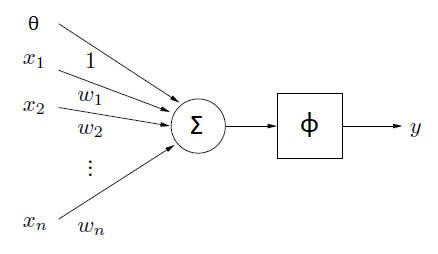
\includegraphics[width=0.8\textwidth]{pics/chapter_neuralnetworks/perzeptron.png}
    \centering
    \caption{Arbeitsweise eines Perzeptrons mit entsprechender Notation aus Definition \ref{def_neuron}.}
    \label{funktionsweise_neuron}
\end{figure}

Bei der Wahl der Funktion $\psi$ gibt es mehrere Möglichkeiten. Wird wie in Minsky\cite{minsky2017perceptrons} die Heavyside-Funktion
\begin{equation*}
    \psi: \RR \rightarrow \RR, \; \; \;
    \psi(x)=\begin{cases}
       1 &, x \geq 0 \\
       0 &, \text{sonst}
    \end{cases}
\end{equation*} 
genutzt, kann das Perzeptron als binärer Klassifikator wie in \ref{abs_linear_trenn} interpretiert werden. Dabei dient $w^Tx+\theta=0$ als trennende Hyperebene. Ist $w^Tx+\theta<0$, so ist $\psi(x)=0$ und $x$ wird der Klasse $K_{-1}$ zugeordnet. Gilt jedoch $w^Tx+\theta \geq 0$ und damit $\psi(x)=1$, so ist der Vektor $x$ der Klasse $K_1$ zugehörig. 

Für ein Klassifikationsproblem, bei dem die Klassen nicht linear trennbar sind, scheitern diese einfachen Perzeptronen. Hier wird oft das zweidimensionale XOR-Problem angeführt, bei denen die Punktmengen $P_{-1}=\{(0,0),(1,1)\}$ und $P_{1}=\{(1,0),(0,1)\}$ getrennt werden sollen. Um solche Aufgaben zu lösen, ist es notwendig, mehrere Perzeptronen geschickt zu verknüpfen, um komplexe Entscheidungsgrenzen zu erhalten.

\section{Multi-Layer-Perzeptron}
\label{MLP_abs}
In dieser Arbeit wird ein Künstliches Neuronales Netz als eine Menge von Perzeptronen, die in gewissen Schichten partitioniert und miteinander verbunden sind, notiert. Diese sogenannten \textit{Multi-Layer-Perzeptronen}, kurz MLP,  gelten als erste tiefe neuronale Netze und sind seit den späten 1980er Gegenstand der Forschung\cite{bourlard1990links,bounds1988multilayer,MLPbook}. Zunächst sind einige Definition notwendig, um eine lesbare Notation des MLPs zu geben.

\begin{defi}[Übertragungsfunktion]
    \label{def_net}
    Für eine gegebene Matrix $W \in \RR^{n \times m}$ und einen Vektor $b \in \RR^m$ ist 
    \[ 
    \Psi^{W,b}: \RR^n \rightarrow \RR^m, \; \; \; x \mapsto W^T x +b
    \]
    als Übertragungsfunktion definiert. Der Vektor $y=\Psi^{W,b}(x) \in \RR^m $ wird als Netzeingabe bezeichnet.
\end{defi}
Hierbei ist $W$ eine Gewichtsmatrix und $b$ ein Biasvektor, welche als freie Parameter fungieren und die Netzeingabe eines Eingabevektors $x \in \RR^n$ auf lineare Art und Weise beeinflussen. Um auch nichtlineare Zusammenhänge darzustellen, werden Aktivierungsfunktionen benutzt.

\begin{defi}[Aktivierungsfunktion]
    \label{def_act_f}
    Eine stetige, monoton steigende und nicht notwendigerweise lineare Funktion $\psi: \RR \rightarrow \RR$ wird als Aktivierungsfunktion bezeichnet.
\end{defi}
Es sei erwähnt, dass auch nicht monotone Aktivierungsfunktionen genutzt werden können, beispielsweise radiale Basisfunktionen\cite{radialbasis}, welche jedoch in dieser Arbeit nicht weiter von Interesse sind.
Typische Aktivierungsfunktionen, die oft verwendet werden, sind die:
\begin{align*}
    \text{Identität}: \; \;\psi(x)&=x, \\
    \text{Logistische Funktion}: \; \;\psi(x)&=\frac{1}{1+\mathrm{e}^{-x}}, \\
    \text{Tangens Hyperbolicus}: \; \;\psi(x)&=\tanh(x), \\
    \text{ReLU (rectified linear unit)}: \; \;\psi(x)&=\max\{0,x\}.
\end{align*}

\begin{bem}
    Ist $\psi$ eine Aktivierungsfunktion, so wird für $x \in \RR^n$ mit 
    \[\psi(x):=\left(\psi(x_1), \ldots, \psi(x_n)\right)^T \in \RR^n
    \]
    der Vektor bezeichnet, welcher sich durch die elementweise Auswertung der Aktivierungsfunktion $\psi$ an den Stellen $x_1, \ldots, x_n$ ergibt. 
\end{bem}

Bei Klassifikationsproblemen wird oft die \textit{Softmax}-Funktion\cite{denker1990transforming} genutzt, welche die gesamte Eingabe berücksichtigt. Im Abschnitt \ref{task_training} wird erläutert, warum sich in diesem Fall die Softmax-Funktion eignet.

\begin{defi}[Softmax]
    Für $x \in \RR^n$ wird die Funktion $\psi: \RR^n \rightarrow (0,1]^n$ mit 
    \[
        \psi(x):=\left(\frac{\mathrm{e}^{x_1}}{\sum_{i=1}^n \mathrm{e}^{x_i}}, \ldots,\frac{\mathrm{e}^{x_n}}{\sum_{i=1}^n \mathrm{e}^{x_i}} \right)^T
    \]
    als Softmax-Funktion definiert. Die Einträge des Vektors $\psi(x)$ summieren sich zu Eins.  
\end{defi}

Für den späteren Trainingsprozess ist es nützlich, die Ableitung der verwendeten Aktivierungsfunktion, sofern sie exisitiert, zur Verfügung zu haben. Zudem ist es möglich, für bestimmte Aktivierungsfunktionen die Ableitung nur mithilfe der verwendeten Funktion zu berechnen.

\begin{lem}
    \begin{itemize}
        \item[(i)] Für die ReLU $\psi(x)=\max\{0,x\}$ gilt
         \[\psi'(x)=\begin{cases}
            0 &, x <0 \\
            1 &, x >0
        \end{cases}. 
        \]
        An der Stelle 0 ist die Ableitung nicht definiert und wird oft mit $\psi'(0)=\frac{1}{2}$ festgelegt.
        \item[(ii)] Für die logistische Funktion $\psi(x)=\frac{1}{1+\mathrm{e}^{-x}}$ gilt
        \[ 
            \psi'(x)=\psi(x)(1-\psi(x)) 
        \]
        für alle $x \in \RR$.
        \item[(iii)] Für den Tangens Hyperbolicus $\psi(x)=\tanh(x)$ gilt
        \[ 
            \psi'(x)=1-\psi^2(x) 
        \]
        für alle $x \in \RR$.
    \end{itemize}
\end{lem}
\begin{proof}
    Einfaches Differenzieren liefert für $(i)$ und $(ii)$ die Resultate. Bei $(iii)$ wird die Darstellung $\tanh(x)=\frac{2}{\mathrm{e}^{2x}+1}$ genutzt und das Differenzieren mittels Quotientenregel liefert die Aussage.
\end{proof}


Ähnlich der Definition des Perzeptron \ref{def_neuron} wird nun eine Schicht als Verknüpfung von Übertragungsfunktion und Aktivierungsfunktion definiert.

\begin{defi}[Neuronenschicht]
    Ist $\Psi^{W,b}$ eine Übertragungsfunktion mit den Parametern $W \in \RR^{n \times m}, b \in \RR^m$ und $\psi$ eine Aktivierungsfunktion, so wird das Paar $(\Psi^{W,b}, \psi)$ als Schicht $\mathcal{S}$ bezeichnet. Für eine Eingabe $x \in \RR^n$ ist die Ausgabe $y \in \RR^m$ der Schicht $\mathcal{S}$ durch
    \[y=\psi \circ \Psi^{W,b}(x)= \psi\left(\Psi^{W,b}(x)\right)
        \] 
        gegeben. Die Komponenten $y_i$ werden für $1 \leq i \leq m$ Neuronen der Schicht $\mathcal{S}$ genannt und gleichen jeweils der Ausgabe eines einfachen Perzeptrons wie in Definition \ref{def_neuron}. Eine Schicht besteht aus $m$ Perzeptronen $\tilde{\Psi}_i$ mit $y_i=\tilde{\Psi}(x_i)=\psi(W_{i,:}^T x+b_i)$ für $1 \leq i \leq m$.
\end{defi}
Im Hinblick auf MLPs werden nun mehrere Schichten so verbunden, dass die Ausgabe einer Schicht $\mathcal{S}_k$ als Eingabe einer darüberliegenden Schicht $\mathcal{S}_{k+1}$ für ein $k \in \mathbb{N}$ dient. Die Anzahl der Neuronen kann dabei von Schicht zu Schicht variieren. Dementsprechend werden die Dimensionen der beteiligten Gewichtsmatrizen $W^{(k)}$ und Biasvektoren $b^{(k)}$ passend gewählt. 
Um die Notation übersichtlich zu halten, bezeichne $\Psi^{W^{(k)},b^{(k)},\psi_{k}}$ die Schicht $\mathcal{S}_k$ mit $\Psi^{W^{(k)},b^{(k)},\psi_{k}}(x):= \psi_{k} \left(\Psi^{W^{(k)},b^{(k)}}(x)\right)$.

\begin{defi}[Multi-Layer-Perzeptron, vgl. gruening]
    Für eine gegebene Anzahl $l \in \mathbb{N}, \; l>1$ von Schichten $\Psi^{W^{(1)},b^{(1)},\psi_{1}}, \ldots, \Psi^{W^{(l)},b^{(l)},\psi_{l}}$ bezeichne $s_l \in \mathbb{N}$ die Anzahl der Neuronen in Schicht $l$. Für eine Eingabe $x \in \RR^{s_0}$ lässt sich die Ausgabe $y \in \RR^{s_l}$ eines Multi-Layer-Perzeptron  $\Lambda_l: \RR^{s_0} \rightarrow \RR^{s_l}, \; x \mapsto y$ mit $l$ Schichten durch
    \[
        y=\Psi^{W^{(l)},b^{(l)},\psi_{l}} \circ \ldots \circ \Psi^{W^{(1)},b^{(1)},\psi_{1}}(x)
    \]
    berechnen. Dabei gelten für die Gewichtsmatrizen die Dimensionsbedingungen
    \[{}_1W^{(1)}=s_0, \; \; {}_2W^{(l)}=s_l, \; \; \forall i \in [l-1]: \; {}_2W^{(i)}={}_1W^{(i+1)}.
        \] 
    Die Eingabeschicht $\mathcal{S}_0$ besitzt keine Parameter $W$ und $b$ und besteht nur aus dem Eingabevektor $x \in \RR^{s_0}$. Die letzte Schicht $\Psi^{W^{(l)},b^{(l)},\psi_{l}}$ wird als Ausgabeschicht bezeichnet. Weiter werden die Schichten $\mathcal{S}_1, \ldots, \mathcal{S}_{l-1}$ als verdeckte Schichten definiert. Die Funktionsauswertung $\Lambda_l(x)$ für eine Eingabe $x$ wird Vorwärtsrechnung, engl. \textit{forward propagation}, genannt.
\end{defi}

\begin{algorithm}
    \caption{Vorwärtsrechnung}\label{alg:ff}
    \begin{algorithmic}
    \Require $ \text{MLP} \; \Lambda_l, \text{Input} \; x_0 \in \RR^n$
    \Ensure $y = \Lambda_l(x) \in \RR^m$
    \State $x=x_0$
    \For{$i=1, \ldots l}$
    \State $u=W^{(i) \,T}x+b^{(i)}$
    \State $x=\psi_i(u)$
    \EndFor
    \State $y=x$
    \end{algorithmic}
\end{algorithm}
    


Das MLP-Modell wird im weiteren Verlauf dieser Arbeit repräsentativ als Künstliches Neuronales Netz bezeichnet. Die Funktionsauswertung eines KNN wird im Algorithmus Vorwärtsrechnung \ref{alg:ff} festgehalten. Das zuvor angesprochene XOR-Problem kann nun beispielsweise mithilfe eines KNN bestehend aus zwei Schichten gelöst werden\cite{Goodfellow-et-al-2016}.
Es lassen sich zwischen Modell- und Hyperparameter von KNN unterscheiden.

\begin{defi}[Hyper- und Modellparameter]
    Sei für $l \in \mathbb{N}$ ein KNN $\Lambda_l$ gegeben. Dann werden die Eingabe- und Ausgabedimension $s_0, s_l$, die Anzahl $l$ der (verdeckten) Schichten sowie die verwendeten Aktivierungsfunktion $\psi_l$ Hyperparameter des neuronalen Netzes genannt.
    Die Gewichtsmatrizen und Biasvektoren mit den entsprechend passenden Abmessungen stellen die Modellparameter $\mathcal{W}:=\{(W^{(i)},b^{(i)}): \; i=1, \ldots, l\}$ des neuronales Netzes dar. 
\end{defi}
Die Hyperparameter werden oft anwendungsspezifisch für das jeweilige Problem gewählt, während die Modellparameter dynamisch in einem Trainingsprozes angepasst werden, sodass die gegebene Aufgabe zufriedenstellend gelöst wird. Wie sies geschieht, wird im folgenden Abschnitt \ref{task_training} erläutert.

\section{Training neuronaler Netze}
\label{task_training}
Künstliche Neuronale Netze gehören zu den typischen Vertretern von maschinellen Lernalgorithmen, welche hinsichtlich einer bestimmten Aufgabe, engl. \textit{task T}, und einem Leistungsmaß, engl. \textit{perfomance P} an der Erfahrung, engl. \textit{experience E} lernen\cite{Goodfellow-et-al-2016}. Dabei ist mit Lernen gemeint, dass das Computerprogramm bezüglich der Aufgabe $T$ sein Leistungsmaß $P$ mit wachsener Erfahrung $E$ schrittweise steigert. Wie in Kapitel \ref{fund} erläutert, gibt es viele verschiedene Aufgaben, wie die Regression, Klassifikation oder Clusterung bestimmter Objekte. 

In den folgenden Abschnitten wird das Klassifikationsproblem im Mittelpunkt stehen. Weiter werden KNNs als Modellschätzer aus der Wahrscheinlichkeitstheorie interpretiert und fundamentale Aussagen wie das \textit{Universal-Approximation-Theroem}\cite{HORNIK1989359} gegeben. Schließlich wird bezüglich der Klassifikationsaufgabe das Training neuronaler Netze erläutert.


\subsection{Neuronale Netze als universelle Schätzer}
\label{NN_estimators_abs}
Beim Klassifikationsproblem müssen bestimmte bedingte Wahrscheinlichkeiten, die in diesem Abschnitt erklärt werden, ermittelt werden. Oft wird dazu die Ausgabeschicht eines KNN als Wahrscheinlichkeit interpretiert und daher KNN als Schätzer der bedingten Wahrscheinlichkeiten eingesetzt. Zunächst werden Klassifikationsfunktion und -problem definiert.
\begin{defi}
    \label{def_classfun}
    Seien die Mengen $D \subset \RR^n$ und $\mathcal{C}=\{c_1, \ldots, c_m\}$ gegeben. Eine Funktion $f: D \rightarrow \mathcal{C}$, welche ein Element aus $D$ einer Klasse $c_i \in \mathcal{C}$ zuordnet, wird Klassifikationsfunktion genannt. Hier gibt es $m \in \mathbb{N}$ verschiedene Klassenlabels. Die Menge $D$ wird abstrakter Datensatz genannt.
\end{defi}

Das Ziel beim Klassifikationsproblem ist die Approximation einer nicht bekannten Klassifikationsfunktion $f:D \rightarrow \mathcal{C}$ durch ein Modell $\tilde{f}: D \rightarrow \mathcal{C}$. 
In dieser Arbeit werden dafür KNNs genutzt, welche als probabilistische Modelle auf folgende Weise genutzt werden. Auf der Ergebnismenge $\Omega= D \times \mathcal{C}$ sei die nicht bekannte gemeinsame (Wahrscheinlichkeits-) Verteilung $p_{Daten}(x,c)$, genannt Datenverteilung, gegeben. Ein Modell soll nun konstruiert werden, welches die a posterior-Verteilung $p_{Daten}(\cdot \; | \; x)$ der Klassen schätzt. 

In dieser Arbeit werden KNN so benutzt, dass die Klassenzugehörigkeit direkt anhand der Eingabe $x \in D$ geschätzt wird. Die Funktion $P_{Daten}: D \rightarrow [0,1]^m$ mit
\begin{equation}
    \label{eq:Pdaten}
    P_{Daten}(x):=\left(p_{Daten}(c_1 \; | \; x), \ldots, p_{Daten}(c_m \; | \; x)\right)^T \in \RR^m
\end{equation} soll für alle $x \in D$ approximiert werden. Dazu wird die Funktion $P_{Modell}: D \rightarrow [0,1]^m$ mit 
\begin{equation}
    \label{eq:Pmodell}
    P_{Modell}(x;\mathcal{W}):=\left(p_{Modell}(c_1 \; | \; x; \mathcal{W}), \ldots, p_{Modell}(c_m \; | \; x; \mathcal{W})\right)^T \in \RR^m
\end{equation}
 für alle $x \in D$ als Approximation genutzt, welche von den Modellparametern $\mathcal{W}$ abhängig ist. Die Klassifikationsfunktion des Modells ergibt sich als
\begin{equation}
    \label{eq:f_modell}
    f_{Modell}(x):= \underset{c \in \mathcal{C}}{\mathrm{argmax}} \; p_{Modell}(c \; | \; x).
\end{equation}

Es stellt sich die Frage, inwiefern das MLP als Modell genutzt werden kann, um beliebige Datenverteilungen $P_{Daten}$ zu approximieren. Folgende Resultate liefern die Antwort.

\begin{satz}[Universal-Approximation-Theroem\cite{gruen}]
    \label{UAT}
    Sei $\psi_1$ eine nichtkonstante, beschränkkte Aktivierungsfunktion und $id: \RR \rightarrow \RR$ die Identität sowie $D \subset \RR^n$ kompakt. Dann existieren für alle $\varepsilon >0$ und stetigen Funktionen $f: D \rightarrow \RR$ Parameter $N \in \mathbb{N}, W^{(1)} \in \RR^{n \times N}, b^{(1)} \in \RR^N$ sowie $W^{(2)} \in \RR^{N \times 1}$, sodass
    \begin{equation}
        \label{UAP_eq}
        \left|f(x)-\Psi^{W^{(2)},0,id} \circ \Psi^{W^{(1)},b^{(1)},\psi_1}(x)\right| < \varepsilon, \; \; \forall x \in D
    \end{equation}
    gilt.
\end{satz}

\begin{proof}
    Ein Beweis kann in Hornik\cite{hornik1991approximation} nachgelesen werden.
\end{proof}

Das Universal-Approximation-Theroem kann ebenfalls auf unbeschränkte und nichtkonstante Funktion $f:D \rightarrow \RR^m$ erweitert werden. Heutzutage wird oft die ReLU-Funktion als Aktivierungsfunktion verwendet\cite{schmidt2020nonparametric,li2017convergence}.

\begin{kor}
    Mit den gleichen Vorraussetzungen wie in Satz \ref{UAT} gilt die Abschätzung \ref{UAP_eq} für $\psi_1(x)=\max\{0,x\}$.
\end{kor}

\begin{proof}
    Siehe Sonoda et. al.\cite{sonoda2017neural}.
\end{proof}

Hinsichtlich der Approximation von beliebigen Funktionen $P_{Daten}$ mithilfe eines neuronalen Netzes mit der Softmax-Funktion als Aktivierungsfunktion liefert Strauß\cite{strauss} folgendes Resultat.

\begin{kor}
    \label{kor_softmax}
    Ein MLP mit zwei Schichten, wobei $\psi_2$ die Softmax-Funktion ist, kann genutzt werden, um stetige Funktionen $f:K \rightarrow [0,1]^m$, welche von einem Kompaktum $K \subset \RR^n$ in eine (Wahrscheinlichkeits)-Verteilung über die Klassen $\mathcal{C}$ abbilden, beliebig genau zu approximieren.
\end{kor}

\begin{proof}
    Siehe \cite{strauss}.
\end{proof}

Die Aussage kann auf das MLP mit beliebig vielen Schichten erweitert werden.
In dieser Arbeit umfasst die Menge $D$ aus Definition \ref{def_classfun} digitalisierte Objekte und ist endlich und damit kompakt. Daher kann wegen Korollar \ref{kor_softmax} das MLP als Modell genutzt werden, um stetige Funktionen $P_{Daten}$ sinnvoll zu approximieren.

\subsection{Optimale Parameterwahl bei neuronalen Netzen}

Wird ein künstliches neuronales Netz als probabilistisches Modell genutzt und sind die Hyperparameter festgelegt, müssen die Modellparameter $\mathcal{W}$ gewählt werden. Um die Approximationsgüte messbar zu machen, wird eine Fehlerfunktion eingeführt, welche mithilfe des Gradientenverfahrens aus Kapitel \ref{fund} durch die Anpassung der Parameter $\mathcal{W}$ in einem Trainingsprozess minimiert werden soll. Im folgenden sei $\Lambda_l$ ein KNN mit der Softmax-Funktion als Aktivierungsfunktion in der Ausgabeschicht, welches als parametrisiertes Modell $f_{Modell}$ wie in \ref{eq:f_modell} genutzt wird.

\begin{defi}[Trainingsmenge]
    Seien $p_{daten}$ eine Datenverteilung und $\Omega=D \times \mathcal{C}$. Dann heißt für ein $k \in \mathbb{N}$ die Menge
    \begin{equation*}
        \mathcal{T}:=\left\{ (x^{(i)},c^{(i)}) \; | \; i \in [k] \right\} \subset \Omega
    \end{equation*}
    Trainingsmenge bestehend aus $k$ Trainingsdaten, welche unabhängig durch $p_{Daten}$ generiert wurde.
\end{defi}

Die Güte des Modells $f_{Modell}$ wird als Likelihood gegeben einer Trainingsmenge $\mathcal{T}$ gemessen und lässt sich als 

\begin{equation}
    \label{eq:likelihood}
    L(\mathcal{T},\mathcal{W}):=\prod_{(x,c) \in \mathcal{T}} p_{Modell}(c \; | \; x; \mathcal{W})
\end{equation}
wie in Bishop\cite{bishop2006pattern} berechnen.
Für eine Trainingsmenge $\mathcal{T}$ soll das Produkt über alle Wahrscheinlichkeiten der korrekten Klassenzugehörigkeiten $c$ gegeben der Eingaben $x$ maximiert werden. Dieser Ansatz wird \textit{Maximum Likelihood-Methode}\cite{ruschendorf2014mathematische} genannt und die Parameterwahl des Modells wird durch eine Lösung des Optimierungsproblems 
\begin{equation}
    \label{eq:opt_likelihood}
     \prod_{(x,c) \in \mathcal{T}} p_{Modell}(c \; | \; x; \mathcal{W}) \rightarrow \max
\end{equation}
gegeben. Dabei sei bemerkt, dass die Optimierung unabhängig von den Hyperparametern vorgenommen wird.

Für ein Trainingspaar $(x,c) \in \mathcal{T}$ bezeichne $t \in \RR^m$ den Zielvektor der Klasse $c$ mit sogenannter (1 aus m)-Kodierung. Die Komponenten von $t=t(x)$ sind
\begin{equation*}
    t_k:= \begin{cases}
        1 &, \text{wenn} \, k=c \\
        0 &, \text{sonst}
    \end{cases}, \; \; \forall k \in [m].
\end{equation*} 
Mit dieser Bezeichnung lässt sich das Optimierungsproblem \ref{eq:opt_likelihood} als Minimierungproblem mithilfe der \textit{negative log likelihood} schreiben.
\begin{defi}[negative log likelihood]
    Seien die Mengen $D$ und  $\mathcal{C}=\{c_1, \ldots, c_m\}$ mit einer dazugehörigen Trainingsmenge $\mathcal{T}$ sowie entsprechende Zielvektoren gegeben. Weiter seien die a posterior Wahrscheinlichkeiten $p_{Modell}(c \; | \; x; \mathcal{W})$ wie in Gleichung \ref{eq:Pmodell} gegeben. Die negative log likelihood ist als Funktion 
    \begin{equation}
        \label{eq:NLL}
        L_{NNL}(\mathcal{T},\mathcal{W}):= -\sum_{(x,c) \in \mathcal{T}}  \sum_{i=1}^m t_i \log \left(p_{Modell}(c_i \; | \; x; \mathcal{W}) \right) 
    \end{equation}
    definiert.
\end{defi}

Das Minimieren der negative log likelihood ist äquivalent zur Maximierung der Likelihood aus \ref{eq:likelihood}, denn es gilt 
\begin{equation*}
    \log \left(\prod_{(x,c) \in \mathcal{T}} p_{Modell}(c \; | \; x; \mathcal{W})\right)= \sum_{(x,c) \in \mathcal{T}} \log \left(p_{Modell}(c \; | \; x; \mathcal{W}) \right)
\end{equation*}
und der natürliche Logarithmus ist monoton steigend. Wird zusätzlich angenommen, dass die Datenverteilung einer Normalverteilung mit konstanter Varianz entspricht, so ist das Maximieren von \ref{eq:likelihood} äquivalent zur Minimierung der mittleren quadratischen Abweichung
\begin{equation*}
    \label{eq:MSE}
    L(\mathcal{T},\mathcal{W})_{MSE}:=\sum_{(x,c) \in \mathcal{T}} \frac{1}{2} ||\hat{c}-t_c||_2^2,
\end{equation*}
wobei $\hat{c}=f_{Modell}(x)$ und $t_c$ der Zielvektor des Datenpaars $(x,c)$ ist, siehe Goodfellow\cite{Goodfellow-et-al-2016}.




\chapter{Gefaltete neuronale Netze}
\label{kap:CNN}

Feed-Forward-Netze gelten als leistungsstarke maschinelle Lernmethoden, da sie so trainiert werden können, um beliebige komplexe Funktionen abhängig von einer vektorwertigen Eingabe zu approximieren. Ist die Dimension der Eingabeschicht jedoch zu groß, treten bei klassischen FFN Probleme hinsichtlich der Paramteranzahl auf. Die Problemstellung \ref{prob:class_image} dieser Arbeit besteht in der Klassifikation digitalisierter Bilder. Wird ein FFN mit $100$ Ausgabeneuronen genutzt und jeder Pixel eines Bildes mit den Abmessungen $1000 \times 1000$ als Merkmal genutzt, so ergeben sich bereits $10^8+100$ freie Parameter. Stehen nur relativ wenige Traingsdaten zur Verfügung, ist die Struktur des FFN zu komplex und dies kann zur Überanpassung führen\cite{caruana2000overfitting,bilbao2017overfitting}. Die Parameteranzahl muss also deutlich reduziert werden. Konzepte wie \textit{Parameter Sharing} und spärliche Konnektivität, engl. \textit{sparse connectivity} erlauben diese Reduktion, vgl. Goodfellow\cite{Goodfellow-et-al-2016} und werden in den folgenden Abschnitten erläutert.

Ein weiterer Nachteil des FFN ergibt sich dadurch, dass Korrelationen von benachbarten Eingabeneuronen, z.B. Bilsegmente wie Kanten oder Ecken, nicht miteinbezogen werden. Es muss also eine Modell entwickelt werden, welches diese lokalen Muster extrahiert und sie miteinander verknüpft. Das Modell sollte zudem äquivariant gegenüber Translationen sein. 

%Schließlich sind beim FFN die Eingabe- und Ausgabedimension fixiert. Eine flexible Wahl diser Hyperparameter ist bei Problemen der Computergrafik oft erwünscht. 

In diesem Kapitel wird erläutert, wie gefaltete neuronale Netze die erwähnten Nachteile von FFN umgehen. CNN sind in der Lage, lokale Muster zu erkennen, sind äquivariant gegenüber Translationen und realisieren Konzepte wie Parameter Sharing, um die Anzahl der freien Parameter drastisch zu reduzieren. So gelingt es, besonders bei Aufgaben der Computergrafik\cite{DBLP:conf/nips/KrizhevskySH12, DBLP:journals/pieee/LeCunBBH98,DBLP:conf/cvpr/CiresanMS12} die Generalisierungsrate gegenüber klassichen FFN zu erhöhen. 

Gefaltete neuronale Netze unterscheiden sich von FFN bei der Berechnung der Übertragungsfunktion. Dazu wird die gefaltete Übertragungsfunktion definiert, welche das Konzept der diskreten Faltung nutzt. Im folgenden Abschnitt \ref{abs:conv_theorie}wird zunächst die Faltung als mathematische Operation eingeführt und deren Zusammenhang zur Fourier-Transformation\cite{werner2011funktionalanalysis} erläutert. Anschließend wird im Abschnitt \ref{abs:conv_def} das CNN-Modell definiert und schließlich im Abschnitt \ref{abs:CNN_train} der Backpropagationsalgorithmus \ref{alg:online_backprop} auf CNN verallgemeinert.

%bei CNNs zu verstehen ist und wie diese Operation bei diesen neuronalen Netzen motiviert wird. In diesem Zusammenhang werden Begriffe wie Merkmalskarten (engl. \textit{feature maps}) und Filter (engl. \textit{kernels}) eingeführt. Des Weiteren wird die Arithmetik der Faltungsoperation für zweidimensionale Eingaben, repräsentiert durch Matrizen, erklärt und das Verfahren \textit{padding} beziehungsweise das Nutzen von \textit{strides} erläutert. Das gesamte Kapitel wird mit konkreten Beispielen begleitet, um die verschiedenen Effekte der Faltungsoperation zu beleuchten.

\section{Die Faltungsoperation}
\label{abs:conv_theorie}
In der Analysis ist die Faltung ein mathematischer Operator und liefert für zwei Funktionen $f$ und $g$ die Funktion $ f \ast g$, wobei mit dem Sternchen die Faltungsoperation gemeint ist.

\begin{defi}[Faltung]\label{allg_faltung}
    Für zwei Funktionen $f,g: \Rnv \rightarrow \mathbb{C}$ ist die Faltung als
    \begin{equation*}
        (f \ast g) (x) := \int_{\Rnv} f(\tau) g(x-\tau) \mathrm{d} \tau
    \end{equation*}
    definiert, wobei gefordert wird, dass das Integral für fast alle $x$ wohldefiniert ist. Für $f,g \in L^1(\RR^n)$ ist dies der Fall.
   \end{defi}

Für die Faltung gelten einige Rechenregeln.

\begin{lem}
    \label{lem:convrules}
    Seien $f,g,h \in L^1(\RR^n)$ und $a \in \mathbb{C}$. Dann gelten
    \begin{align*}
         (i) \; \; &f \ast g = g \ast f \; \; &( \text{Kommutativität}) \\
         (ii) \; \; &f \ast (g \ast h) = (f \ast g) \ast h  \; \;& (\text{Assoziativität}) \\
         (iii) \; \; &f \ast (g+h) = (f+g) \ast h \; \; &(\text{Distributivität}) \\ 
         (iv) \; \; &a(f \ast g) = (af) \ast g = f \ast (ag) \; \; &(\text{Assoziativität mit skalarer Multiplikation}) 
    \end{align*}
\end{lem}

\begin{proof}
    Eine Beweis dieser Rechenregeln kann in Werner\cite{werner2011funktionalanalysis} nachgelsen werden.
\end{proof}

%Bei klassischen neuronalen Netzen, siehe Kapitel \ref{classicNN} werden Eingabedaten durch eine Verkettung von affinen Transformationen verarbeitet. Typischerweise wird die Eingabe als Vektor dargestellt und  mit einer Matrix multipliziert, gegebenenfalls mit einem Biasvektor manipuliert und schließlich so die Ausgabe generiert. Bilder-, Audio- oder Videoaufnahmen besitzen jedoch mehrere Merkmale in unterschiedlichen Achsen. Oft sind solche Eingabedaten im Bereich des Machine-Learnings als mehrdimensionale Arrays abgelegt, welche eine oder mehrere Achsen repräsentieren, wobei die Ordnung dieser eine Rolle spielt. Bei digitalisierten Bildern sind das bespielsweise die Höhe und Breite des Bildes, bei Audioaufnahmen gibt es nur eine Achse, und zwar die Zeitachse. Hinzu kommen Kanalachsen als weitere Verfeinerung der Daten, zum Beispiel besitzen RGB-Farbbilder drei Kanäle der Farben rot, grün und blau. 

%Diese speziellen Eigenschaften können bei affinen Transformationen nicht berücksichtigt werden. Alle Merkmale sowie Achsen werden gewissermaßen gleich behandelt und die wesentliche topologische Struktur kann so nicht zum Vorteil ausgenutzt werden. Hier soll nun die sogenannte diskrete Faltung Abhilfe schaffen.
In der digitalen Signal- und Bildverarbeitung werden meist diskrete Funktionen analysiert und daher die diskrete Faltung genutzt, bei der statt der Intgration eine Summation auftaucht. Die Regeln aus Lemma \ref{lem:convrules} gelten analog.

\begin{defi}[Diskrete Faltung]\label{disk_faltung}
    Für zwei Funktionen $f,g: D \rightarrow \mathbb{C}$ mit einem diskreten Definitionsbereich $D \subseteq \mathbb{Z}^n$ ist die diskrete Faltung als
    \begin{equation*}
        (f \ast g) (n) := \sum_{k \in D} f(k) g(x-k)
    \end{equation*}
    definiert. Hier wird über dem gesamten Definitionsbereich $D$ summiert. Ist $D$ beschränkt, werden $f$ beziehungsweise $g$ durch Nullen fortgesetzt.  
\end{defi}

Ist für $f,g: D \rightarrow \mathbb{C}$ der Definitionsbereich $D$ endlich, so können die Funktionen als zeitdiskrete Signale $f=(f_0, \ldots, f_{n-1})^T \in \mathbb{C}^{n}$ und $g=(g_0, \ldots, g_{n-1})^T \in \mathbb{C}^{n}$ aufgefasst werden. %Durch das Fortsetzen mit Nullen besitzen die Vektoren $f$ und $g$ die gleiche Länge. 
In diesem Fall kann die Faltung als Matrix-Vektor-Produkt mit einer zyklischen Matrix ausgedrückt werden. 

\begin{defi}[Zyklische Matrix, vgl. Gray\cite{gray2006toeplitz}]
    Eine quadratische Matrix heißt zyklisch im Vektor $a=(a_0, \ldots, a_{n-1})^T \in \RR^n$, wenn sie die Gesatlt
    \begin{equation*}
        \mathrm{zyk}(a):=
        \begin{pmatrix}
            a_0 & a_{n-1} &a_{n-2} &\ldots &a_1 \\ 
            a_1 & a_0 &a_{n-1} & \ldots &a_2 \\
            a_2 & a_1 &a_0 & \ldots &a_3 \\
             &\ddots &\ddots &\ddots & \\
            a_{n-1} &a_{n-2} &a_{n-3} &\ldots &a_0
        \end{pmatrix}
    \end{equation*}
    besitzt.
\end{defi}    
    
\begin{bem}
Für ein zeitdiskrete Signal $f=(f_0, \ldots, f_{n-1})^T \in \mathbb{C}^{n}$ sei $F=\mathrm{zyk}(f)$ die zyklische Matrix im Vektor $f$. Sei weiter $g=(g_0, \ldots, g_{n-1})^T \in \mathbb{C}^{n}$. Dann lässt sich mit
    \begin{equation*}
        (F g)_k=\sum_{j=0}^{n-1}  f_{k-j} g_j,  \; \; k=0, \ldots, n-1
    \end{equation*}
    die diskrete Faltung von $f$ und $g$ darstellen. Dabei werden Indizies außerhalb von $0, \ldots, n-1$ zyklisch durch Modulo-Rechnung ($\mathrm{mod} \; n)$ in den gültigen Indexbereich abgebildet.
\end{bem}

In Hinblick auf die Klassifikation von digitalisierten Bildern, dargestellt als Matrizen, wird die Matrixfaltung mit sogenannten quadratischen Kernen $K \in \RR^{k \times k}$ mit ungeradem $k \in \mathbb{N}$ definiert.
 
%Um die Notation einfach zu halten, sei ein Kern $K$ ebenfalls eine $h \times b$ - Matrix, indem $K$ mit Nullen aufgefüllt wird.

%\begin{defi}[Zweidimensionale Faltung]
    %Sei $X \in \RR^{h \times b}$ und $K \in \RR^{k \times k}$. Das Ergebnis der zweidimensionalen Faltung ist die Matrix $Y= X \ast K \in \RR^{h \times b}$ mit

%    \begin{equation}
%        \label{eq:2dmatrixconv}
%        Y_{i,j}= \sum_{p \in [k]} \sum_{q \in [k]} X_{p,q} K_{p-i+3,q-j+3}.
%    \end{equation}
%    Dabei besitzt $Y$ die selben Abmessungen wie $X$. 
%\end{defi}

\begin{defi}[Matrixfaltung, vgl. \cite{gruening}] \label{def:matrix_faltung}
    Für gegebene Matrizen $X \in \RR^{h \times b}$ und $K \in \RR^{k \times k}$ sei $u=\lfloor k/2  \rfloor$.
    %\begin{equation*}
    %   h_l=\begin{cases}
    %       \lfloor k_h/2  \rfloor &, k_h \, \text{ungerade} \\
    %       k_h/2-1 &, \text{sonst}
    %    \end{cases}, \; \; 
    %    w_l=\begin{cases}
    %        \lfloor k_w/2 \rfloor &, k_w \, \text{ungerade} \\
    %        k_w/2 -1 &, \text{sonst}    
    %    \end{cases}.
    %\end{equation*} 
    Die zweidimensionale Faltung  $Y=X \ast K \in \RR^{h \times w}$ ist als 
    \begin{equation}
        \label{eq:matrix_faltung}
        (Y)_{i,j}:=\sum_{l=-u}^{u} \sum_{m=-u}^{u} X_{i+l,j+m} K_{l+u+1, m+u+1}\; \; \forall i \in [h], j \in [b]
    \end{equation} mit $X_{i,j}=0$ für $i \notin [h]$ und $j \notin [b]$ definiert. In der Literatur wird dieses Auffüllen mit Nullen am Rand von $X$ mit \textit{zero padding} bezeichnet. In dieser Definition besitzt das Ergebnis $Y$ der Faltung die gleichen Abmessungen wie $X$.
\end{defi}

Bei gefalteten neuronalen Netzen wird oft eine Reduktion der Dimensionen angestrebt. Dafür werden natürliche Zahlen als Schrittweiten, engl. \textit{strides}, genutzt.
\begin{bem}\label{bem_strides}
    Für Schrittweiten $s_h, s_b \in \mathbb{N}$ ergibt sich die reduzierte zweidimensionale Faltung $Y=X \ast K$ zu
    \begin{equation*}
        (Y)_{i,j}:=\sum_{l=-u}^{u} \sum_{m=-u}^{u} X_{i \cdot s_h +l,j \cdot s_b +m} K_{l+u+1, m+u+1}\; \; \forall i \in [\lceil h/s_h \rceil], j \in [\lceil b/s_b \rceil].
    \end{equation*}
    Für $s_h=s_b=1$ ergibt sich die Standardvariante wie in \ref{eq:matrix_faltung}.
    \end{bem}

\section{CNN Architektur}

Beim maschinellen Lernen sind Eingabedaten oft als mehrdimensionale Arrays abgelegt, welche eine oder mehrere Achsen repräsentieren, wobei die Ordnung dieser eine Rolle spielt. Bei digitalisierten Bildern sind das bespielsweise die Höhe und Breite des Bildes, welche als Raumachsen bezeichnet werden. Hinzu kommen Kanalachsen, zum Beispiel besitzen Grauwert-Bilder einen Farbkanal, während RGB-Farbbilder drei Kanäle der Farben rot, grün und blau besitzen. Dementsprechend werden Grauwert-Bilder wie in Definition \ref{def:image} nun als dreidimensionale Arrays $X \in [0,1]^{h \times b \times 1}$ dargestellt. Dies erlaubt die Definition der gefalteten Übertragungsfunktion, wie in Gruening\cite{gruening}

\begin{defi}[Gefaltete Übertragungsfunktion]
    \label{eq:convlogit}
    Sei ein vierdimensionales Array $K \in \RR^{z_{out} \times z_{in} \times k \times k}$ und ein Biasvektor $b \in \RR^{z_{out}}$ gegeben. Die Funktion 
    \begin{equation*}
        \Psi_{conv}^{K,b}: \RR^{\cdot \times \cdot \times z_{in}} \rightarrow \RR^{\cdot \times \cdot\times z_{out}}
    \end{equation*}
    mit
    \begin{equation*}
        \Psi_{conv}^{K,b}(X)_{:,:,q}:= \sum_{p=1}^{z_{in}} \alpha_p\left(K_{q,p,:,:} \ast X_{:,:,p} \right) +b_q \; \forall q \in [z_{out}]
    \end{equation*}
    wird gefaltete Übertragungsfunktion bezeichnet. Mit $\ast$ ist die Matrixfaltung wie in Definition \ref{def:matrix_faltung} gemeint und mit $\cdot$ werden beliebige Raumachsen bezeichnet. Die Skalare $\alpha_p$ sind lernbare Parameter. In dieser Arbeit gelte $\alpha_p=1$ für alle $p \in [z_{in}]$.
\end{defi}


\begin{bem}
    Ist $\psi: \RR \rightarrow \RR$ eine Aktivierungsfunktion wie in Definition \ref{def_act_f}, so wird für $X \in \RR^{\cdot \times \cdot \times z}$ mit 
    \[\psi(X)_{i,j,:}:=\left(\psi(X_{i,j,1}), \ldots, \psi(X_{i,j,z})\right)^T \in \RR^z \; \; \forall i \in [{}_1 X], j \in [{}_2 X] 
    \]
    der Vektor bezeichnet, welcher sich durch die elementweise Auswertung der Aktivierungsfunktion $\psi$ ergibt.
\end{bem}

Ähnlich der Definition \ref{def:NNlayer} wird nun eine Faltungsschicht als Verknüpfung von gefalteter Übertragungsfunktion und Aktivierungsfunktion definiert.

\begin{defi}[Faltungsschicht]
    \label{def:convlayer}
    Ist $\Psi_{conv}^{K,b}$ eine gefaltete Übertragungsfunktion und $\psi$ eine Aktivierungsfunktion, so wird das Paar $(\Psi_{conv}^{K,b}, \psi)$ als Faltungsschicht $\mathcal{S}_{conv}$ bezeichnet. Für eine sogenannte Eingabekarte $X \in \RR^{\cdot \times \cdot \times z_{in}}$ ist die Ausgabe $Y \in \RR^{\cdot \times \cdot \times z_{out}}$ der Schicht $\mathcal{S}_{conv}$ durch
    \[Y=\psi \circ \Psi_{conv}^{K,b}(X)= \psi\left(\Psi_{conv}^{K,b}(X)\right)
        \] 
        gegeben. Die Matrizen $Y_{:,:,p}$ werden für $1 \leq p \leq z_{out}$ Merkmalskarten genannt. Weiter bezeichne $\Psi_{conv}^{K^{},b^{},\psi_{}}$ die Faltungsschicht $\mathcal{S}_{conv}$ mit $\Psi_{conv}^{K^{},b^{},\psi_{}}(X):= \psi_{} \left(\Psi_{conv}^{K^{},b^{}}(X)\right)$.
\end{defi}

Bei CNN werden sogenannte \textit{Pooling}-Schichten verwendet, um die Dimensionen der Raumachsen neben dem zero padding weiter zu verkleinern und das Modell robuster gegenüber Überanpassung zu machen. Dazu werden Pooling-Funktionen eingesetzt, welche unabhängig voneinander auf Merkmalskarten operieren und so die Rechenkomplexität des Modells reduzieren. Es ist sinnvoll, symmetrische Pooling-Funktionen $T$ zu wählen, für die die Bedingung
\begin{equation*}
    \forall \pi \in S_n \; \forall x \in \RR^n: T(x_1, \ldots, x_n)=T(x_{\pi(1)}, \ldots, x_{\pi(n)})
\end{equation*}
gilt. Mögliche Pooling-Funktionen sind 
\begin{alignat*}{2}
    \text{Maximum}: \; \;&T(x_1, \ldots x_n) &&= \max\{x_1, \ldots x_n\},\\
    \text{Mittelwert}: \; \;&T(x_1, \ldots, x_n) &&= \frac{1}{n} \sum_{i=1}^n x_i. 
 \end{alignat*}
Heutzutage wird oft die von Weng et. al.\cite{weng1992cresceptron} eingeführte Max-Pooling-Schicht benutzt.
Für den späteren Trainingsprozess ist es nützlich, die Ableitung der verwendeten Pooling-Funktionen, sofern sie existiert, zur Verfügung zu haben. Für den Mittelwert $T$ gilt $\nabla T=\frac{1}{n} \textbf{1}$. Ist $T$ die Maximum-Funktion so ergibt sich

\begin{equation*}
    \frac{\partial T}{\partial x_i}= \begin{cases}
        1 , \; \text{falls}  \; \forall j \neq i: \; x_i >x_j \\
        0 , \; \text{falls}  \; \exists j \neq i: \; x_i <x_j
    \end{cases}
\end{equation*}
mit der Konvention, dass für $x_1=x_2= \ldots=x_n$ die Ableitung auf $\frac{1}{2}
$ gesetzt wird. Pooling-Schichten werden wieder durch Schrittweiten parametrisiert.

\begin{defi}[Pooling-Schicht, vgl. Grüning \cite{gruening}]
    Seien $p_h, p_b \in \mathbb{N}$ und $T$ eine Pooling-Funktion. Die Funktion 
    \begin{equation*}
        \Psi_{pool,T}^{p_h,p_b}: \RR^{\cdot \times \cdot \times z} \rightarrow \RR^{\cdot \times \cdot\times z}
    \end{equation*}
    mit
    \begin{equation*}
        \Psi_{pool,T}^{p_h,p_b}(X)_{i,j,l}:= \mathop{T}_{\begin{subarray}{l}(i-1) \cdot p_h < i' \leq \min\{i \cdot p_h, {}_1 X\} \\ 
        (j-1) \cdot p_w < j' \leq \min\{j \cdot p_w, {}_2 X\}\end{subarray}} (X_{i',j',l})  
    \end{equation*}
    für alle  $i \in [\lceil {}_1 X/p_h \rceil], j \in [\lceil {}_2 X/p_w \rceil]$ und $l \in [z]$ wird Pooling-Schicht genannt. Die Schrittweiten $p_h, p_b \in \mathbb{N}$ werden subsampling-Faktoren genannt.
\end{defi}

Pooling-Schichten verdichten also Information von Eingabedaten, welche sich lokal in Fenstern der Größe $p_h \times p_b$ befinden und reduzieren so die Raumdimension. In dieser Arbeit wird das Maximum-Pooling oder Mittelwert-Pooling benutzt. Für andere Pooling-Funktion sei auf Yu et. al.\cite{yu2014mixed} verwiesen.
Die Idee bei CNN besteht nun darin, Faltungsschichten mit Pooling-Schichten zu kombinieren und schließlich ein FFN wie in Definition \ref{def:MLP} anzuknüpfen.
Dazu wird für allgemeine mehrdimensionale Arrays die Flatten-Schicht definiert.

\begin{defi}
    \label{def:flatten}
    Sei $X \in \RR^{n_1 \times n_2 \times n_3}$. Dann wird die Funktion $T_f:\RR^{n_1 \times n_2 \times n_3} \rightarrow \RR^{n_1 \cdot n_2 \cdot n_3}$ mit 
    \begin{equation*}
        T_f(X)_{(i-1) \cdot (n_2 \cdot n_3)+(j-1) \cdot n_3+k}:= X_{i,j,k}, \; \; \forall i \in [n_1],\; j \in [n_2],\; k \in [n_3]
    \end{equation*}
    Flatten-Funktion genannt. Die multidimensionale Eingabe wird also in einen Vektor umgewandelt.
\end{defi}

Dies erlaubt die Definition des CNN-Modells als Kombination aus Faltungsschichten, Pooling-Schichten und Neuronenschichten des MLP aus Kapitel \ref{kap:NN}. 
\begin{defi}(Gefaltetes Neuronales Netz)
    Seien $h, w, z_{in}, z_{out}, l ,c \in \mathbb{N}$ und Schichten $\Psi^{W^{(1)},b^{(1)},\psi_{1}}, \ldots, \Psi^{W^{(l)},b^{(l)},\psi_{l}}$ sowie Faltungsschichten $\Psi_{conv}^{K^{(1)},b^{(1)},\psi_{1}}, \ldots, \Psi_{conv}^{K^{(l)},b^{(l)},\psi_{l}}$ gegeben. Die Vorwärtsrechnung eines CNN lässt sich als Komposition
    \begin{equation}
        \label{eq:CNN_for}
        y=\Psi^{W^{(l)},b^{(l)},\psi_{l}} \circ \ldots \circ \Psi^{W^{(1)},b^{(1)},\psi_{1}} \circ T_f \circ \Psi_{conv}^{K^{(c)},b^{(c)},\psi_{c}} \circ \ldots \circ \Psi_{conv}^{K^{(1)},b^{(1)},\psi_{l}}(X)
    \end{equation} 
    darstellen. Dabei seien wieder die Dimensionen der Parameter passend gewählt, sodass die Komposition wohldefiniert ist. In (\ref{eq:CNN_for}) können zwischen den Faltungsschichten Pooling-Schichten $\Psi_{pool,T}^{p_h,p_b}(X)$ geschaltet werden.
\end{defi}
Auch CNN bestehen aus Hyper- und Modellparametern.

\begin{defi}[Hyper- und Modellparameter von CNN]
    Die Eingabe- und Ausgabedimensionen $h, b, z_{in}, z_{out}$, die Anzahl $c$ der Faltunsschichten, dei Anzahl $l$ der Neuronenschichten, die Dimensionen der Kerne, die Schrittweiten bei der Faltung bzw. dem Pooling sowie die verwendeten Aktivierungs- und Poolingfunktionen sind Hyperparameter des CNN.
    Die Kerne, Gewichtsmatrizen und Biasvektoren mit den entsprechend passenden Abmessungen stellen die Modellparameter $\mathcal{W}:=\{(W^{(i)},b^{(i)}): \; i=1, \ldots, l\}$ und $\mathcal{W}_{conv}:=\{(K^{(i)}, b^{(i)}): \; i=1, \ldots, c\}$ des CNN dar. 
\end{defi}
Die Hyperparameter werden wieder anwendungsspezifisch für das jeweilige Problem gewählt und die Modellparameter während des Trainingsprozesses angepasst. 


\section{Backpropagation bei CNN}
\label{abs:CNN_train}
Der Backpropagationsalgorithmus \ref{alg:online_backprop} soll nun für das CNN-Modell verallgemeinert werden. 
Als Fehlerfunktion wird wieder die mittlere quadratische Abweichung (\ref{eq:MSE})
genutzt. 
Die Abstiegsrichtungen für die Schichten des FFN wurden bereits im vorherigen Kapitel \ref{kap:NN} hergeleitet. Es müssen nun Gradienten innerhalb der Faltungsschichten beziehungsweise Pooling-Schichten berechnet werden. Die Einträge der Eingabe- und Merkmalskarten, in Zukunft einfach Karten genannt, können als Neuronenaktivierungen interpretiert werden. Weiter werden zur Vereinfachung die trainierbaren Gewichte der Kerne in Zukunft mit $w_{i,j}^{(l)}$ bezeichnet. Gemeint ist also das Gewicht zwischen Neuron $i$ auf Schicht $l-1$ und Neuron $j$ der Schicht $l$ bezeichnet. Weiter sei $y_{i}^{(l-1)}$ die Aktivierung des Neurons $i$ der Schicht $l-1$ und $\delta_j^{(l)}$ sei der lokale Fehler des Neurons $j$ der Schicht $l$. Die Funktion $\psi$ repräsentiert eine Aktivierungsfunktion, Pooling-Funktion oder Flatten-Funktion, je nachdem auf welcher Schicht sie benutzt wird.

Die Gradienten werden wieder komponentenweise berechnet.
Angenommen, $l$ ist eine Faltungsschicht. Die Aktivierung einer Merkmalskarte $j$ an der Stelle $(x,y)$ lässt sich mit der Matrixfaltung, siehe \ref{def:matrix_faltung}, \ref{eq:convlogit}, als
\begin{equation}
    y_j^{(l)}(x,y) =\psi \left(\sum_{i \in [z_{in}]} \sum_{(u,v) \in F} y_i^{(l)}(x+u,y+u)\,  w_{j,i}^{(l)}(u,v) +b_j^{(l)}\right)
\end{equation}   
schreiben. Es ist zu beachten, dass $(x,y)$ ein Pixel der Karte $j$ meint. Dabei ist $F=\{(u,v): \; 0\leq u,v <k\}$ und $k$ die Dimension der Kerns.
Das Gewicht des Kerns von der Karte $i$ zur Karte $j$ an der Stelle $(u,v)$ ist mit $w_{j,i}(u,v)$ bezeichnet. Der Gradient ergibt sich als Summe über das Produkt der jeweilgen Positionen $(x,y)$ der Merkmalskarte $j$ und dem lokalen Fehler $\delta^{(l)}_j$, also
\begin{equation}
    \label{eq:CNN_K_grad}
    \Delta w_{j,i}^{(l)}(u,v)= -\lambda \, \sum_{(x,y)} \left( y_i^{(l-1)}(x+u,y+v) \delta_j^{(l)}(x,y)\right)
\end{equation}
Der Zusammenhang in Gleichung (\ref{eq:CNN_K_grad}) ist in Abbildung \ref{abb:error_conv} grafisch dargestellt. Analog ergibt sich für den Schwellwert

\begin{equation*}
    \Delta b_j^{(l)}= -\lambda \, \sum_{(x,y)} \delta_j^{(l)}(x,y).
\end{equation*}
Die Berechnung des lokalen Fehlers $\delta_{j}^{(l)}$ der Schicht $l$ ist abhängig von der Schicht $l+1$.
$V_k=\sum_{j} w_{k,j}^l z_j +b^l_k$ 

\section{Anwendung bei der Ziffernerkennung}
In diesem Abschnitt wird ein CNN zur Klassifikation von Grauwert-Bildern aus einem konkreten Datensatz vorgestellt. Der MNIST-Datensatz\cite{DBLP:journals/pieee/LeCunBBH98} bietet $60.000$ Trainingsbilder handgeschriebener Ziffern und $10.000$ Testbilder, welche jeweils durch menschliches Wissen annotiert sind. Dieser Datensatz gilt als typischer Benchmark zur Klassifikation von Ziffern und wird im weiteren Verlauf dieser Arbeit genutzt. Jedes einzelne Bild besteht aus $28 \times 28$ Pixeln, welche jeweils einen Grauwert zwischen 0 und 1 annehmen, vgl. Abbildung \ref{mnistpic}. Ein Bild wird als $X \in [0,1]^{28 \times 28 \times 1}$ und ein Trainingspaare als $(X,c)$ mit $c \in \{0, \ldots, 9\}$ bezeichnet. 

\begin{figure}[h]
    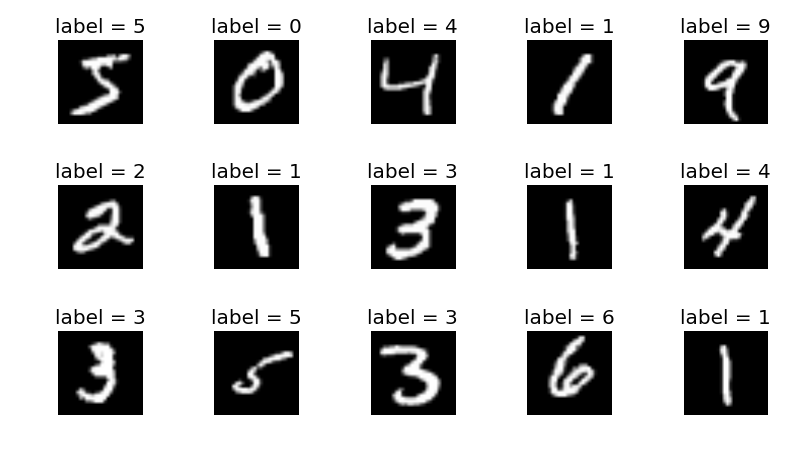
\includegraphics[width=0.8\textwidth]{pics/chapters/CCN/mnist.png}
    \centering
    \caption{Beispielbilder, vgl. \cite{DBLP:journals/pieee/LeCunBBH98} aus der öffentlichen MNIST-Datenbank. Zu sehen sind handgeschriebene Ziffern und zugehörige Annotationen.}
    \label{mnistpic}
\end{figure}

Es wird ein CNN mit zwei Faltungsschichten $C^1$ und $C^2$ mit der logistischen Aktivierungsfunktion $\psi$ genutzt. Die Ausgabe der Schicht $C^1$ umfasst sechs Merkmalskarten und die Ausgabe der Schicht $C^2$ zwölf Merkmalskarten. Zur Faltung werden quadratische $5 \times 5$ -Kerne verwendet. Außerdem werden zwei Pooling-Schichten $P^1$ und $P^2$mit den Schrittweiten $p_h=p_b=2$ und der Mittelwert-Funktion genutzt. Anschließend wird ein FFN mit 10 Ausgabeneuronen angekoppelt, sodass dessen Aktivierung zur Klassifikation der Eingabe genutzt werden kann. Die Architektur, ähnlich dem Le-Net-5-Modell\cite{DBLP:journals/pieee/LeCunBBH98}, ist in Abbildung \ref{abb_CNN_arch} dargestellt. Dabei sind

\begin{itemize}
    \item $X$ ein Grauwert-Bild der Größe $h=b=28$,
    \item $K^1 \in \RR^{6 \times 1 \times 5 \times 5}$ der Kern der Schicht $C^1$,
    \item $b^1 \in \RR^6$ der Biasvektor der Schicht $C^1$,
    \item $K^2 \in \RR^{12 \times 6 \times 5 \times 5}$ der Kern der Schicht $C^2$,
    \item $b^2 \in \RR^{12}$ der Biasvektor der Schicht $C^2$,
    \item $W \in \RR^{192 \times 10}$ die Gewichtsmatrix der Neuronenschicht,
    \item $b \in \RR^{10}$ der Biasvektor der Neuronenschicht,
    \item $y \in \RR^{10}$ die Ausgabe des CNN. 
\end{itemize}

Im Folgenden wird der Online-Backpropagationsalgorithmus \ref{alg:online_backprop_CNN} verwendet, um das CNN zu trainieren. Dieser besteht zunächst aus der Initialisierung und der Vorwärtsrechnung. Zur Übersicht wird im Folgenden eine komponentenweise Schreibweise genutzt.

\section*{Vorwärtsrechnung}

Alle Biasvektoren werden als Nullvektor initialisiert. Zur Initialisierung der Gewichte wird die Xavier-Initialisierung \ref{def:xavier} genutzt, also

\begin{alignat*}{2}
    K^{1}_{p,1}(u,v) &\sim  \mathcal{N} \left(0, \frac{2}{5 \cdot 5 \cdot (1+6)}\right), \; \; && p \in [6],\\
    K^{2}_{q,p}(u,v) &\sim  \mathcal{N} \left(0, \frac{2}{5 \cdot 5 \cdot (6+12)}\right),\; \; && q \in [12], p \in [6],\\
    W(i,j) &\sim \mathcal{N} \left(0, \frac{2}{192+10}\right), \; \; &&\forall i \in [192], \forall j \in [10].
\end{alignat*}
Die Parameteranzahl ist damit 
\begin{equation*}
    \underbrace{(5 \cdot 5 +1) \cdot 6}_{\text{Gewichte in $C^1$}}+\underbrace{(5 \cdot 5 \cdot 6+1) \cdot 12}_{\text{Gewichte in $C^2$}}+\underbrace{(192+1 \cdot 10)}_{\text{Gewichte im FFN}}=3898.
\end{equation*}
 Sei $X \in \RR^{28 \times \times 1}$ das Eingabebild und $\psi$ die logistische Funktion. In der Schicht $C^1$ werden sechs Merkmalskarten 

\begin{align}
    \label{eq:C1_forw}
    \begin{split}
    C_p^1 &= \psi(X \ast K_{p,1}^1+b_p^1 \mathbf{1}) \\
    C_p^1(i,j)&=\psi \left(\sum_{u=0}^4 \sum_{v=0}^4 X(i+u,j+v) \cdot K_{p,1}^1(u,v) +b_p^1\right)
    \end{split}
\end{align}
für $1 \leq p \leq 6$ berechnet. Mit $\mathbf{1} \in \RR^{24 \times 24}$ ist die Matrix gemeint, deren Einträge nur Einsen sind. Die Matrixfaltung $\ast$ wird ohne zero padding genutzt und daher reduziert sich die Raumdimension. Es gilt $C^1_p \in \RR^{24 \times 24 \times 1}$. Anschließend folgen das Mittelwert-Pooling $P^1$ mit
\begin{equation}
    \label{eq:P1_forw}
    P^1_p(i,j) =\frac{1}{4} \sum_{u=0}^1 \sum_{v=0}^1 C_p^1(2i-u, 2j-v), \; i,j \in [12]
\end{equation}
für $1 \leq p \leq 6$ und die zweite Faltungsschicht $C^2$, welche zwölf Merkmalskarten
\begin{align}
    \label{eq:C2_forw}
    \begin{split}
        C_q^2 &= \psi \left( \sum_{p=1}^6 P_p^1 \ast K_{q,p}^2 + \mathbf{1} b_q^2\right) \\
        C_q^2(i,j) &= \psi \left( \sum_{p=1}^6 \sum_{u=0}^4 \sum_{v=0}^4 P^1_p(i+u,j+v) \cdot K^2_{q,p}(u,v) +b_q^2\right)
    \end{split}
\end{align}
für $1 \leq q \leq 12$ berechnet. Die Matrixfaltung $\ast$ wird wieder ohne zero padding genutzt und daher reduziert sich die Raumdimension.
Es gilt $C_q^2 \in \RR^{8 \times 8 \times 1}$. Es folgt das Mittelwert-Pooling $P^2$ mit
\begin{equation}
    \label{eq:P2_forw}
    P_q^2(i,j)= \frac{1}{4} \sum_{u=0}^1 \sum_{v=0}^1 C_p^1(2i-u, 2j-v), \; i,j \in [4]
\end{equation}
für $1 \leq q \leq 12$. Es gilt $P^2\in \RR^{4 \times 4 \times 12}$. Diese zwölf $4 \times 4$- Matrizen werden durch die Flatten-Funktion $T_f$ aus Definition \ref{def:flatten} in einen Vektor $f \in \RR^{4 \cdot 4 \cdot 12}$ umgewandelt. Dies sei durch
\begin{equation}
    \label{eq:f_forw}
    f=T_f(P^2)
\end{equation}
beschrieben. 
Die Umkehrung wird mit
\begin{equation}
    \label{eq_f_ford_inv}
    P^2=T_f^{-1}(f).
\end{equation}
bezeichnet.
Die Ausgabe des FFN ergibt sich schließlich zu
\begin{equation}
    \label{eq:y_forw}
    y=\psi(W^T f +b).
\end{equation}
und der mittlere quadratische Fehler lautet
\begin{equation}
    \label{eq:E_forw}
    E_{X}=\frac{1}{2} \sum_{k=1}^{10} \left(y(k)-t(k)\right)^2,
\end{equation}
wobei $t=t(X,c)$ der Zielvektor des Datenpaars $(X,c)$ ist.

\section*{Backpropagation}
Zuerst werden die Gradienten bezüglich der Gewichtsmatrix und Biasvektor der Neuronenschicht des FNN berechnet. Es gilt
\begin{align}
    \begin{split}
        \Delta W(j,k) &= -\lambda \, \frac{\partial E}{\partial W(j,k)}\\
                       &= -\lambda \, \frac{\partial L}{\partial y(k)} \cdot \frac{\partial y(k)}{\partial W(j,k)}\\
                       &=-\lambda \, (y(k)-t(k)) \cdot \frac{\partial}{\partial W(j,k)} \psi \left(\sum_{j=1}^{192} W(j,k) f(j)+b(k)\right)\\
                       &=-\lambda \, (y(k)-t(k)) \cdot y(k)(1-y(k)) \cdot f(j).
     \end{split}
\end{align}
Mit $\delta^{\text{FFN}}(k)=(y(k)-t(k)) \cdot y(k)(1-y(k))$ für $1 \leq k \leq 10$ lässt sich $\Delta W$ als dyadisches Produkt  
\begin{align*}
    \Delta W(j,k)&=-\lambda \, \left(\delta^{\text{FFN}}(k) \cdot f(j) \right) \\
    \Rightarrow  \Delta W&=-\lambda \,\left(f \otimes (\delta^{\text{FFN}})^T\right)   
\end{align*}
darstellen. Analog gilt
\begin{equation*}
\Delta b= -\lambda \delta^{\text{FFN}}.
\end{equation*}
Um $ \Delta K_{q,p}$ in $C^2$ zu bestimmen, sind zunächst die lokalen Fehler der darüberliegenden Schicht zu ermitteln. Der lokale Fehler $\delta^f \in \RR^{}$ in der Flatten-Schicht lautet
\begin{align*}
    \delta^F(j) &= - \lambda \, \frac{\partial E}{\partial f} \\
                &= - \lambda \, \sum_{k=1}^{10} \frac{\partial E}{\partial y(k)} \cdot \frac{\partial y(k)}{f(j)} \\
                &= - \lambda \, (y(k)-t(k)) \cdot \frac{\partial}{\partial f(j)} \psi \left(\sum_{j=1}^{192} W(k,j) f(j) +b(k)\right) \\
                &=- \lambda \, \sum_{k=1}^{10} (y(k)-t(k)) \cdot y(k)(1-y(k)) \cdot W(k,j) \\
                &=-\lambda \,\sum_{k=1}^{10} \delta^{\text{FFN}}(k) \cdot W(k,j) \\
                \Rightarrow \delta^F &= -\lambda \, W^T \delta^{\text{FFN}}
\end{align*}
In der Pooling-Schicht $P^2$ sind keine Gradienten zu bestimmen, da diese nicht von den Modellparametern abhängt. Mit
\begin{equation*}
    \delta^{P^2}=T_f^{-1}(\delta^F) \in \RR^{4 \times 4 \times 12}
\end{equation*}
folgt mit der Mittelwert-Funktion $
\phi:\RR^4 \rightarrow \RR^4$ und $\nabla \phi=\frac{1}{4} \mathbf{1}$ das Upsampling
\begin{align*}
    \delta^{C^2}_q(i,j)&= \delta^{P^2}_q\left( \lceil i/2 \rceil, \lceil j/2 \rceil\right) \cdot \nabla \phi(\lceil i/2 \rceil)\\
    &=\delta^{P^2}_q\left( \lceil i/2 \rceil, \lceil j/2 \rceil\right) \cdot \frac{1}{4} \; \; \forall i,j \in [8] 
\end{align*}
für $1 \leq q \leq 12$. Es gilt $\delta^{C^2} \in \RR^{8 \times 8 \times 12}$. Nun kann $\Delta K^2_{q,p}$ an einer Stelle $(u,v)$ berechnet werden.
\begin{align*}
    \Delta K^2_{q,p}(u,v) &= -\lambda \, \frac{\partial E}{\partial K^2_{q,p}(u,v)} \\
                          &= -\lambda \, \sum_{i=1}^8 \sum_{j=1}^8 \frac{\partial E}{\partial C^2_q(i,j)} \cdot \frac{\partial C^2_q(i,j)}{\partial K_{q,p}^2(u,v)} \\
                          &= -\lambda \, \sum_{i=1}^8 \sum_{j=1}^8 \delta_q^{C^2}(i,j) \cdot \frac{\partial}{ K^2_{q,p}(u,v)} \psi \left( \sum_{p=1}^6 \sum_{u=0}^4 \sum_{v=0}^4 P^1_p(i+u,j+v) \cdot K_{q,p}(u,v) +b_q^2\right) \\
                          &= -\lambda \, \sum_{i=1}^8 \sum_{j=1}^8 \delta_q^{C^2}(i,j) \cdot C_q^2(i,j)\left(1-C_q^2(i,j)\right) \cdot P^1_p(i+u,j+v)
\end{align*}
für $1 \leq q \leq 12, 1 \leq p \leq 6$.
Mit 
\begin{equation*}
    \delta^{C^2}
\end{equation*}
%Im Folgenden werden konkrete Beispiele für verschiedene zweidimensionale Faltungen, welche in dieser Arbeit im Fokus stehen, gegeben. Dabei sind die Eingabe $X \in \RR^{h \times w}$ und der Filter $K \in \RR^{k_h \times k_w}$ immer als Matrizen zu verstehen. Das Ergebnis der Faltung $S= X \ast K$ wird als Merkmalskarte bezeichnet. Es sei angemerkt, dass oft $k_h=k_w$ sowie $k_h$ ungerade gewählt wird, z.B. $k_h=3$ oder $k_h=5$. Die Größe der Merkmalskarte wird durch die Parameter
%\begin{itemize}
%    \item $h,w$: Die Höhe und Breite der Eingabe,
%    \item $k_h, k_w$: Die Abmessungen des Filters,
%   \item $s_h, s_w$: Die Wahl der strides, 
%   \item $p_h, p_w$: Die Größe des zero paddings
%\end{itemize}
%beeinflusst. Mit zero padding ist gemeint, dass künstliche Nullen um Randpixel der Eingabe $X$ eingefügt werden, damit die Berechnung mit dem Filter um jene Pixel gelingt. Ein Beispiel für das Verwenden von zero padding wird in Abbildung \ref{abb_simplematrixconv_padding} gezeigt. In Abbildung \ref{abb_simplematrixconv} ist die Berechnung einer einfachen zweidimensionalen Matrixfaltung dargestellt. Ein vorher festgelegter Filter (grau) bewegt sich über die Eingabe (blau) und berechnet jeweils die Einträge der Ausgabe(grün). 

\begin{figure}[h]
    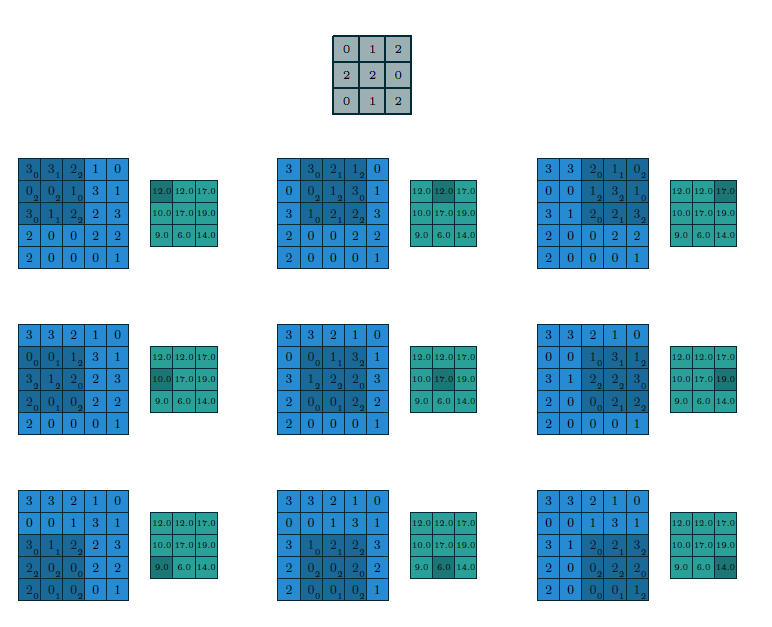
\includegraphics[width=0.8\textwidth]{pics/abb_simpleconv}
    \centering
    \caption{Es wird die Merkmalskarte $S \in \RR^{3 \times 3}$ mit den Parametern ${h,w=5}, k_h=k_w=3, s_h=s_w=1$ und $p_h=p_w=1.$}
    \label{abb_simplematrixconv}
\end{figure}

\begin{figure}[h]
    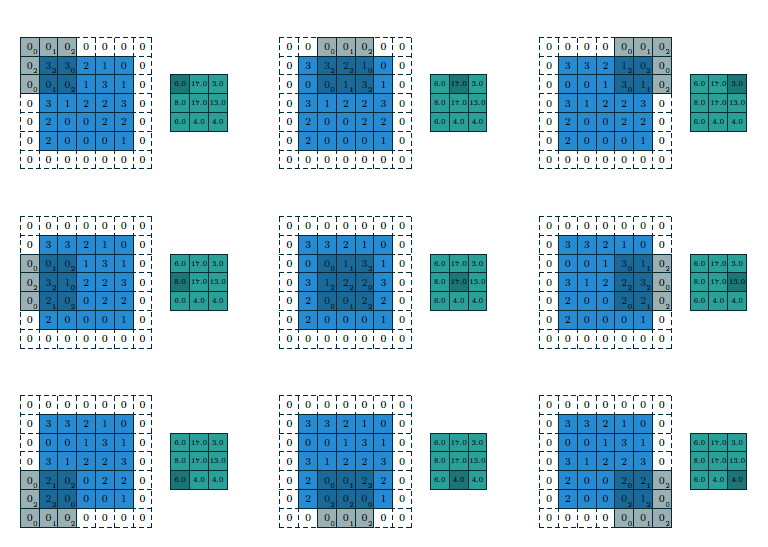
\includegraphics[width=0.8\textwidth]{pics/abb_simplecov_padding}
    \centering
    \caption{Es wird die Merkmalskarte $S \in \RR^{3 \times 3}$ mit den Parametern ${h,w=5}, k_h=k_w=3, s_h=s_w=2$ und $p_h=p_w=1$ berechnet.}
    \label{abb_simplematrixconv_padding}
\end{figure}



\section{Motivation der Faltung}
..
Sie nutzt wichtige Konzepte zur Optimierung von Machine-Learning-Verfahren wie spärliche Konnektivität (engl. \textit{sparse connectivity}), \textit{Parameter Sharing} und \textit{äquivariante Repräsentation}, vgl. \cite{goodfellow}. Spärliche Konnektivität bedeutet, dass Neuronen auf einer Schicht $\mathcal{s}_{l+1}$ nur durch wenige Neuronen der Schicht $\mathcal{S}_l$ beeinflusst wird. Dies ist bei CNNs typisch, da meist die verwendeten Filter viel kleiner als die Eingabe ist. Noch mehr erklären + Abbildung

Mit Parameter Sharing ist die Nutzung von gleichen Parametern für mehrere Funktionen im neuronalen Netz gemeint. In herkömmlichen Feed-Forward-Netzen wird jedes Element der Gewichtsmatrizen für die Berechnung der Aktivierungen der jeweiligen Schichten verwendet. Anschließend werden diese Gewichte dann nicht mehr gebraucht. Im Zusammenhang von CNNs bedeutet Parameter Sharing während der Faltungsoperation, dass nur eine bestimmte Menge von Parametern erlernt werden müssen
Noch mehr erklären + Abbildung


%\chapter{Die Faltung}
In diesem Kapitel wird erläutert, wie die Faltung (engl. \textit{convolution}) bei CNNs zu verstehen ist und wie diese Operation bei diesen neuronalen Netzen motiviert wird. In diesem Zusammenhang werden Begriffe wie Merkmalskarten (engl. \textit{feature maps}) und Filter (engl. \textit{kernels}) eingeführt. Des Weiteren wird die Arithmetik der Faltungsoperation für zweidimensionale Eingaben, repräsentiert durch Matrizen, erklärt und das Verfahren \textit{padding} beziehungsweise das Nutzen von \textit{strides} erläutert. Das gesamte Kapitel wird mit konkreten Beispielen begleitet, um die verschiedenen Effekte der Faltungsoperation zu beleuchten.

\section{Die Faltungsoperation}
In der Analysis ist die Faltung ein mathematischer Operator und liefert für zwei Funktionen $f$ und $g$ die Funktion $ f \ast g$, wobei mit dem Sternchen die Faltungsoperation gemeint ist.

\begin{defi}[Faltung]\label{allg_faltung}
    Für zwei Funktionen $f,g: \Rnv \rightarrow \mathbb{C}$ ist die Faltung als
    \begin{equation*}
        (f \ast g) (x) := \int_{\Rnv} f(\tau) g(x-\tau) \mathrm{d} \tau
    \end{equation*}
    definiert, wobei gefordert wird, dass das Integral für fast alle $x$ wohldefiniert ist.
   \end{defi}

Bei klassischen neuronalen Netzen, siehe Kapitel \ref{classicNN} werden Eingabedaten durch eine Verkettung von affinen Transformationen verarbeitet. Typischerweise wird die Eingabe als Vektor dargestellt und  mit einer Matrix multipliziert, gegebenenfalls mit einem Biasvektor manipuliert und schließlich so die Ausgabe generiert. Bilder-, Audio- oder Videoaufnahmen besitzen jedoch mehrere Merkmale in unterschiedlichen Achsen. Oft sind solche Eingabedaten im Bereich des Machine-Learnings als mehrdimensionale Arrays abgelegt, welche eine oder mehrere Achsen repräsentieren, wobei die Ordnung dieser eine Rolle spielt. Bei digitalisierten Bildern sind das bespielsweise die Höhe und Breite des Bildes, bei Audioaufnahmen gibt es nur eine Achse, und zwar die Zeitachse. Hinzu kommen Kanalachsen als weitere Verfeinerung der Daten, zum Beispiel besitzen RGB-Farbbilder drei Kanäle der Farben rot, grün und blau. 

Diese speziellen Eigenschaften können bei affinen Transformationen nicht berücksichtigt werden. Alle Merkmale sowie Achsen werden gewissermaßen gleich behandelt und die wesentliche topologische Struktur kann so nicht zum Vorteil ausgenutzt werden. Hier soll nun die sogenannte diskrete Faltung Abhilfe schaffen.

\begin{defi}[Diskrete Faltung]\label{disk_faltung}
    Für zwei Funktionen $f,g: D \rightarrow \mathbb{C}$ mit einem diskreten Definitionsbereich $D \subseteq \mathbb{Z}^n$ ist die diskrete Faltung als
    \begin{equation*}
        (f \ast g) (n) := \sum_{k \in D} f(k) g(x-k)
    \end{equation*}
    definiert. Hier wird über dem gesamten Definitionsbereich $D$ summiert. Ist $D$ beschränkt, werden $f$ beziehungsweise $g$ durch Nullen fortgesetzt. 
   \end{defi}

Besonders bei der Bildverarbeitung wird oft die diskrete Faltung als lineare Operation verwendet. 

\begin{defi}[Matrixfaltung, vgl. \cite{gruening}] \label{matrix_faltung}
    Für gegebene Matrizen $X \in \RR^{h \times w}$ und $K \in \RR^{k_h \times k_w}$ seien 
    \begin{equation*}
        h_l=\begin{cases}
           \lfloor k_h/2  \rfloor &, k_h \, \text{ungerade} \\
           k_h/2-1 &, \text{sonst}
        \end{cases}, \; \; 
        w_l=\begin{cases}
            \lfloor k_w/2 \rfloor &, k_w \, \text{ungerade} \\
            k_w/2 -1 &, \text{sonst}    
        \end{cases}.
    \end{equation*} 
    Die Matrixfaltung $K \ast X \in \RR^{h \times w}$ ist als 
    \begin{equation}
        \label{matrix_faltung_op}
        (K \ast X)_{i,j}:=\sum_{l=-h_l}^{\lfloor k_h/2  \rfloor} \sum_{m=-w_l}^{\lfloor k_w/2 \rfloor} K_{l+h_l+1, m+w_l+1} X_{i+l,j+m} \; \; \forall i \in [h], j \in [w]
    \end{equation} mit $X_{i,j}=0$ für $i \notin [h]$ und $j \notin [w]$ definiert.
    \end{defi}

\begin{bem}\label{bem_strides}
    Die Matrixfaltung kann durch viele weitere Parameter genauer spezifiziert werden. Sogannte \textit{strides} bestimmen die Reduktion bei der Faltung von $X$ in der Höhe $h$ beziehungsweise Breite $w$. Für strides $s_h, s_w \in \mathbb{N}$ ist die Matrixfaltung als
    \begin{equation*}
        (K \ast X)_{i,j}:=\sum_{l=-h_l}^{\lfloor k_h/2  \rfloor} \sum_{m=-w_l}^{\lfloor k_w/2 \rfloor} K_{l+h_l+1, m+w_l+1} X_{i \cdot s_h +l,j \cdot s_w +m} \; \; \forall i \in [h], j \in [w].
    \end{equation*}
    Für $s_h=s_w=1$ ergibt sich die Standardvariante wie in \ref{matrix_faltung_op}.
    \end{bem}

Im Folgenden werden konkrete Beispiele für verschiedene zweidimensionale Faltungen, welche in dieser Arbeit im Fokus stehen, gegeben. Dabei sind die Eingabe $X \in \RR^{h \times w}$ und der Filter $K \in \RR^{k_h \times k_w}$ immer als Matrizen zu verstehen. Das Ergebnis der Faltung $S= X \ast K$ wird als Merkmalskarte bezeichnet. Es sei angemerkt, dass oft $k_h=k_w$ sowie $k_h$ ungerade gewählt wird, z.B. $k_h=3$ oder $k_h=5$. Die Größe der Merkmalskarte wird durch die Parameter
\begin{itemize}
    \item $h,w$: Die Höhe und Breite der Eingabe,
    \item $k_h, k_w$: Die Abmessungen des Filters,
    \item $s_h, s_w$: Die Wahl der strides, 
    \item $p_h, p_w$: Die Größe des zero paddings
\end{itemize}
beeinflusst. Mit zero padding ist gemeint, dass künstliche Nullen um Randpixel der Eingabe $X$ eingefügt werden, damit die Berechnung mit dem Filter um jene Pixel gelingt. Ein Beispiel für das Verwenden von zero padding wird in Abbildung \ref{abb_simplematrixconv_padding} gezeigt. In Abbildung \ref{abb_simplematrixconv} ist die Berechnung einer einfachen zweidimensionalen Matrixfaltung dargestellt. Ein vorher festgelegter Filter (grau) bewegt sich über die Eingabe (blau) und berechnet jeweils die Einträge der Ausgabe(grün). 

\begin{figure}[h]
    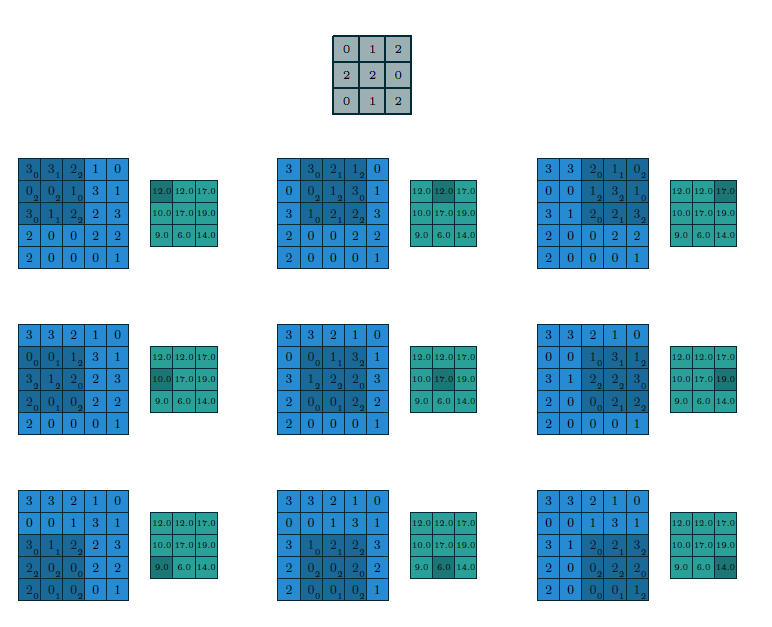
\includegraphics[width=0.8\textwidth]{pics/abb_simpleconv}
    \centering
    \caption{Es wird die Merkmalskarte $S \in \RR^{3 \times 3}$ mit den Parametern ${h,w=5}, k_h=k_w=3, s_h=s_w=1$ und $p_h=p_w=1.$}
    \label{abb_simplematrixconv}
\end{figure}

\begin{figure}[h]
    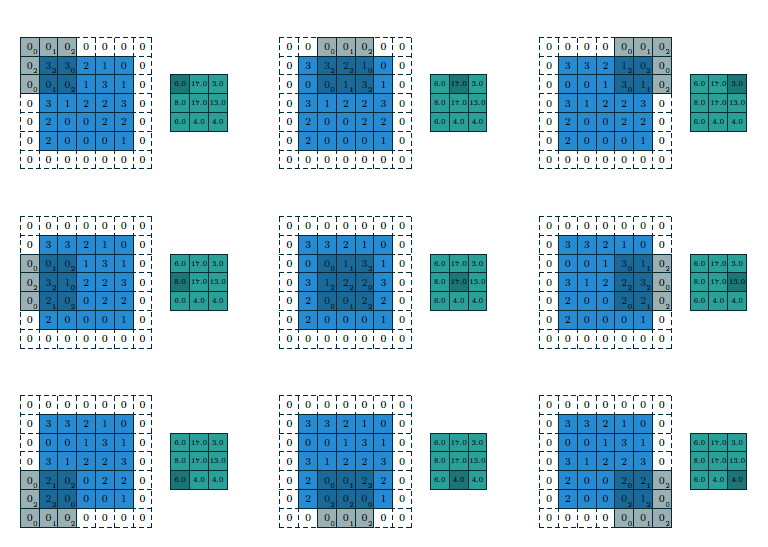
\includegraphics[width=0.8\textwidth]{pics/abb_simplecov_padding}
    \centering
    \caption{Es wird die Merkmalskarte $S \in \RR^{3 \times 3}$ mit den Parametern ${h,w=5}, k_h=k_w=3, s_h=s_w=2$ und $p_h=p_w=1$ berechnet.}
    \label{abb_simplematrixconv_padding}
\end{figure}



\section{Motivation der Faltung}
..
Sie nutzt wichtige Konzepte zur Optimierung von Machine-Learning-Verfahren wie spärliche Konnektivität (engl. \textit{sparse connectivity}), \textit{Parameter Sharing} und \textit{äquivariante Repräsentation}, vgl. \cite{goodfellow}. Spärlicher Konnektivität bedeutet, dass die Ausgabeeinheit auf einer bestimmten Schicht nur durch wenige Eingabeeinheiten beeinflusst wird. Dies ist bei CNNs typisch, da meist die verwendeten Filter viel kleiner als die Eingabe ist. Noch mehr erklären + Abbildung

Mit Parameter Sharing ist die Nutzung von gleichen Parametern für mehrere Funktionen im neuronalen Netz gemeint. In herkömmlichen Feed-Forward-Netzen wird jedes Element der Gewichtsmatrizen für die Berechnung der Aktivierungen der jeweiligen Schichten verwendet. Anschließend werden diese Gewichte dann nicht mehr gebraucht. Im Zusammenhang von CNNs bedeutet Parameter Sharing während der Faltungsoperation, dass nur eine bestimmte Menge von Parametern erlernt werden müssen
Noch mehr erklären + Abbildung



\chapter{Weiteres Kapitel}
Hier wird dies und das vorgestellt. Unter anderem Fußnoten.\footnote{Dies ist eine Fußnote.}
\section{Umgebungen und Formeln}
\begin{defi}\label{defi1}
 \dots\ heißt \ac{rnn}. 
\end{defi}
\begin{bem}\label{bem1}
Bei jeder weiteren Verwendung der Abkürzung wird nur die Kurzform angezeigt: \ac{rnn}.
\end{bem}
\begin{bem}\label{bem2}
Die Verwendung des Symbolverzeichnisses ist analog der des Abkürzungsverzeichnisses, siehe \ac{cm}.
\end{bem}
\begin{annahme}\label{annahme1}
Eine kluge Annahme \dots
\end{annahme}
\begin{hsatz}\label{hsatz1}
Ein kluger Hilfssatz \dots
\end{hsatz}
\begin{satz}\label{satz1}
Ein kluger Satz \dots
\end{satz}
\begin{kor}\label{kor1}
Ein kluges Korollar \dots
\end{kor}
\begin{prop}\label{prop1}
Eine kluge Proposition \dots
\end{prop}
\begin{problem}\label{problem1}
Ein schweres Problem \dots
\end{problem}
\begin{bsp}\label{bsp1}
Ein anschauliches Beispiel \dots
\end{bsp}



\begin{defi}\label{defi2}
Seien $a,b\in\mathbb{C}$ definiere 
\begin{equation}\label{eq1}
a+b
\end{equation}
als  \dots
\end{defi}

Auf Formeln kann nun verwiesen werden (siehe \eqref{eq1}). Formeln können natürlich auch im normalen Text $a^2+b^2=c^2$ auftauchen. 


\begin{empheq}[box=\colorbox{mycolor},right=\empheqrbrace \text{ohne Sinn}]{align}
a^2+b^2&=c^2\\
f&=b-a
\end{empheq}
\section{Aufzählung und Nummerierung}
Für Literaturvereichnisse siehe Kapitel~\ref{ch:bib}, eine einfache Aufzählung geht so:
\begin{itemize}
 \item Eins
 \item Zwei
 \item Viele
\end{itemize}


\section{Tabellen}
\begin{table}[ht]
 \dots\ gibt es viele verschiedene, z.\,B.\ Tab.~\ref{tab:reservoir_segmentlabelling} und Tab.~\ref{tab:dlv_restr_all}. 
\caption{Einfache Tabelle}
\label{tab:reservoir_segmentlabelling}
\centering
  \begin{tabular}{ccrr}
        \toprule
             Column 1 & Column 2 & Column 3 & Column 4 \\
            \midrule
            Nein & Softmax & \SI{85,0}{\%} & \cellcolor{hellgrau} \SI{87,0}{\%} \\
            Nein & Linear & \cellcolor{hellgrau} \SI{88,8}{\%} & \SI{85,9}{\%} \\
            Ja & Softmax & \SI{80,0}{\%} & \cellcolor{hellgrau} \SI{89,1}{\%} \\
            Ja & Linear& \SI{84,6}{\%} & \cellcolor{hellgrau} \SI{89,8}{\%} \\
            \bottomrule
  \end{tabular}
\end{table} 

\begin{table}[ht]
\caption{Nicht mehr ganz so einfache Tabelle}\label{tab:dlv_restr_all}
\centering
 \begin{tabular}{llcccccc}
  \hline\noalign{\smallskip}
  	&source prior				&\multicolumn{2}{c}{\texttt{abs}}&\multicolumn{2}{c}{\texttt{prior}} & \multicolumn{2}{c}{\texttt{da}}\\	
	&source posterior 			&\texttt{path}&	\texttt{ctc}&   \texttt{path}&	\texttt{ctc}&\texttt{path}&\texttt{ctc}\\
	\noalign{\smallskip}
	\hline
	\noalign{\smallskip}
	\multirow{ 2}{*}{gAP}	&\texttt{normed}	&94.81&	94.89&	95.36&	\textbf{95.42}&	94.99&	95.04\\
				&\texttt{unnormed}	&94.77&	&	91.73&	91.87&	92.58&	\\%\hline
	\noalign{\smallskip}
	\multirow{ 2}{*}{mAP}	&\texttt{normed}	&89.71&	\textbf{89.90}&	89.58&  89.76&	89.63&89.82	\\
				&\texttt{unnormed}	&89.42&	&	88.59&	88.89&	89.13&	\\
	\noalign{\smallskip}
	\multirow{ 2}{*}{gNDCG}	&\texttt{normed}	&96.72&	96.78&	96.78&	\textbf{96.83}&	96.73&96.77	\\
				&\texttt{unnormed}	&96.69&	&	96.34&	96.41&	96.46	&\\
	\noalign{\smallskip}
	\multirow{ 2}{*}{mNDCG}	&\texttt{normed}	&90.77&	\textbf{90.97}&	90.66&  90.85&	90.70&90.89 \\
				&\texttt{unnormed}	&90.61&	&	89.96&	90.25&	90.36& \\	
	\hline
 \end{tabular}
\end{table}



\section{Bilder}
\subsection{Einzelnes Bild}
\begin{figure}[ht]
\centering
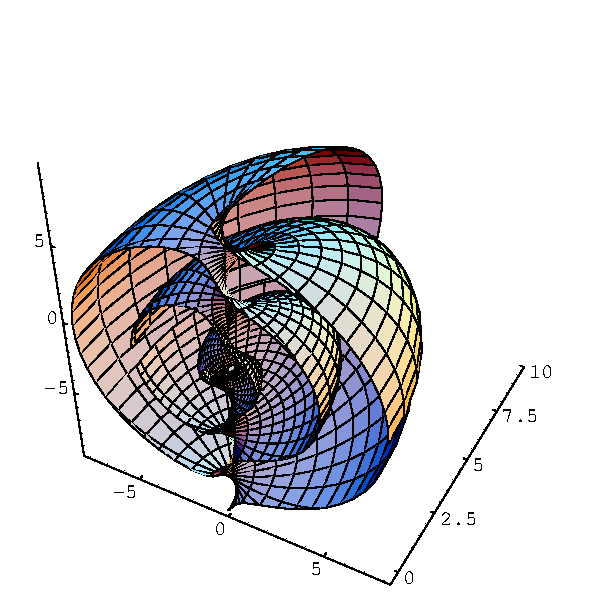
\includegraphics[width=0.5\textwidth]{pics/SCHNECKE}
\caption{Vektorgrafiken sind toll. Scrolle mal in mich rein!}
\label{fig:schnecke}
\end{figure}

Das ist Text. Das ist Text. Das ist Text über Abb.~\ref{fig:schnecke}. Das ist Text.\footnote{Dieser Textteil
ist von wesentlicher Bedeutung}

\subsection{Mehrere Bilder}
\begin{figure}[h!t]
\centering
\begin{subfigure}{0.4\textwidth}
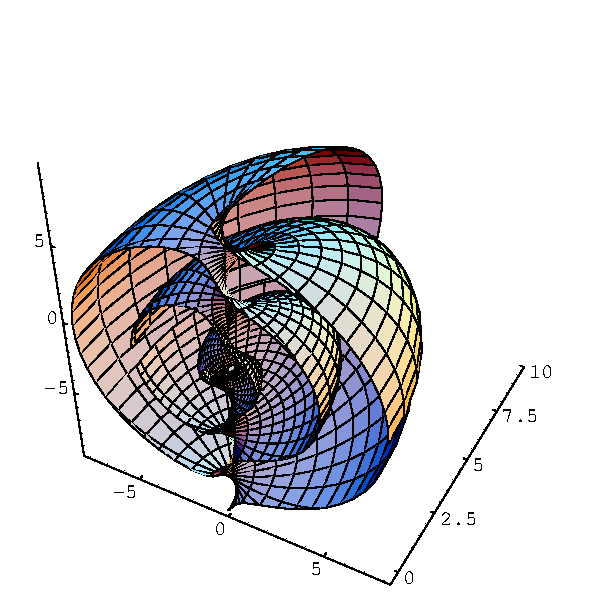
\includegraphics[width=\textwidth]{pics/SCHNECKE}
\subcaption{Schnecke 1}
\label{fig:schnecke:a}
\end{subfigure}
\qquad
\begin{subfigure}{0.4\textwidth}
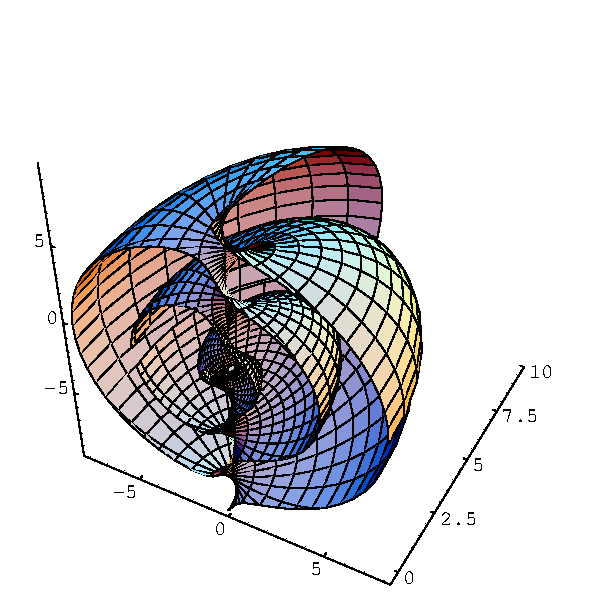
\includegraphics[width=\textwidth]{pics/SCHNECKE}
\subcaption{Schnecke 2}
\label{fig:schnecke:b}
\end{subfigure}
\caption{Vergleich verschiedener Schnecken}
\label{fig:seam}
\end{figure}

Die Schnecke aus Abb.~\ref{fig:schnecke:a} ist hübscher anzusehen als die aus Abb.~\ref{fig:schnecke:b}.

\section{TikZ}
TikZ bietet ein mächtiges Werkzeug Grafiken selber zu erzeugen.
\subsection{Einfache Grafiken}
Es gibt viele, viele Tutorials und Beispiele die leicht im Internet zu finden sind. Aber ein Beispiel sei an dieser Stelle trotzdem eingefügt, siehe Abb.~\ref{fig:tikz}.
\begin{figure}[ht]
\centering
\begin{tikzpicture}[minimum size=5mm,inner sep=0pt]
\node (v1) at (1,.5) [circle,fill=white,draw] {};
\node (v2) at (1.75,.5) [circle,fill=white,draw] {};
\node (v3) at (2.5,.5) [circle,fill=white,draw] {};
\node (v4) at (3.25,.5) [circle,fill=white,draw] {};
\node (v5) at (4,.5) [circle,fill=white,draw] {};
\begin{scope}[on background layer]
\node (vA) [fit=(v1)(v2)(v3)(v4)(v5), minimum width=2cm, inner sep=2pt,fill=white,draw,rounded corners=5pt] {};
\end{scope}
\node (t1) at (0,.5) [] {$\textbf{v}$};
\node (t2) at (1.5,1.25) [] {$Q(\textbf{h}^1|\textbf{v})$};
\node (t3) at (3.5,1.25) [] {$P(\textbf{v}|\textbf{h}^1)$};

\node (h1) at (1,2) [circle,fill=white,draw] {};
\node (h2) at (1.75,2) [circle,fill=white,draw] {};
\node (h3) at (2.5,2) [circle,fill=white,draw] {};
\node (h4) at (3.25,2) [circle,fill=white,draw] {};
\node (h5) at (4,2) [circle,fill=white,draw] {};
\begin{scope}[on background layer]
\node (hA) [fit=(h1)(h2)(h3)(h4)(h5), minimum width=2cm, inner sep=2pt,fill=white,draw,rounded corners=5pt] {};
\end{scope}
\node (t4) at (0,2) [] {$\textbf{h}^1$};
\node (t5) at (1.5,2.75) [] {$Q(\textbf{h}^2|\textbf{h}^1)$};
\node (t6) at (3.5,2.75) [] {$P(\textbf{h}^1|\textbf{h}^2)$};

\draw[thick,->] (hA.300) -- (vA.60);
\draw[thick,->,dotted] (vA.120) -- (hA.240);

\node (h6) at (1,3.5) [circle,fill=white,draw] {};
\node (h7) at (1.75,3.5) [circle,fill=white,draw] {};
\node (h8) at (2.5,3.5) [circle,fill=white,draw] {};
\node (h9) at (3.25,3.5) [circle,fill=white,draw] {};
\node (h10) at (4,3.5) [circle,fill=white,draw] {};
\begin{scope}[on background layer]
\node (hB) [fit=(h6)(h7)(h8)(h9)(h10), minimum width=2cm, inner sep=2pt,fill=white,draw,rounded corners=5pt] {};
\end{scope}
\node (t7) at (0,3.5) [] {$\textbf{h}^2$};
\node (t8) at (3.5,4.25) [] {$P(\textbf{h}^2,\textbf{h}^3)$};

\draw[thick,->] (hB.300) -- (hA.60);
\draw[thick,->,dotted] (hA.120) -- (hB.240);

\node (h11) at (1,5) [circle,fill=white,draw] {};
\node (h12) at (1.75,5) [circle,fill=white,draw] {};
\node (h13) at (2.5,5) [circle,fill=white,draw] {};
\node (h14) at (3.25,5) [circle,fill=white,draw] {};
\node (h15) at (4,5) [circle,fill=white,draw] {};
\begin{scope}[on background layer]
\node (hC) [fit=(h11)(h12)(h13)(h14)(h15), minimum width=2cm, inner sep=2pt,fill=white,draw,rounded corners=5pt] {};
\end{scope}
\node (t9) at (0,5) [] {$\textbf{h}^3$};

\draw[thick,<->] (hB) -- (hC);
\end{tikzpicture}
\caption{Beispiel eines mit TikZ erzeugten Bildes}
\label{fig:tikz}
\end{figure}
\subsection{Graphen und ähnliches}
Wer keine Lust hat z.\,B. Achsenbeschriftungen eines Matlab-Plots auf Font etc. des \LaTeX -Dokuments anzupassen, kann Datenreihen auch einfach mittels TikZ darstellen, siehe dazu Abb.~\ref{fig:ohstats}. Es ist natürlich auch möglich aus z.\,B. Matlab oder Gnuplot Tikz Grafiken zu exportieren!
\begin{figure}[ht]
\centering
\begin{tikzpicture}
		\begin{axis}[width=0.9\textwidth,height=0.3\textheight,
			xtick={0,25,50,75,100,125,150,175,200},
			x tick label style={/pgf/number format/1000 sep=},
			xlabel={Epochs},
			y tick label style={/pgf/number format/1000 sep=},
			ylabel={LBL-Error},
			enlarge x limits=0.0,
			ymin = 0.0,
			ymax = 0.5]		
			\addplot[mark=none,red] table[x=x, y=prime] {tikz/ohdata.txt}; \addlegendentry{System 1}
			\addplot[mark=none,black] table[x=x, y=fixed] {tikz/ohdata.txt}; \addlegendentry{System 2}
			\addplot[mark=none,yellow] table[x=x, y=sma] {tikz/ohdata.txt}; \addlegendentry{System 3}
			\addplot[mark=none,green] table[x=x, y=med] {tikz/ohdata.txt}; \addlegendentry{System 4}
			\addplot[mark=none,blue] table[x=x, y=big] {tikz/ohdata.txt}; \addlegendentry{System 5}
		\end{axis}
\end{tikzpicture}
\caption{Datenreihen mittels TikZ visualisiert}
\label{fig:ohstats}
\end{figure}

\chapter{Ein letztes Kapitel}
\begin{kor}\label{kor2}
Wird f\"{u}r die Festlegung  \dots
\end{kor}
\section{Weiteres Korollar}
In diesem Abschnitt  \dots
\begin{kor}\label{kor3}
Wird f\"{u}r die Festlegung  \dots
\end{kor}

\begin{bem}\label{bem3}
Eine vollst\"{a}ndige  \dots
\end{bem}

\section{Pseudocode}
In vielen Fällen ist es notwendig, Programmteile als Pseudocode darzustellen. Algorithmus \ref{alg:pseudo} stellt ein einfaches Beispiel dar. Es gibt weitere Pakete zur Darstellung von Pseudocode, \texttt{algorithm} + \texttt{algpseudocode} sei an dieser Stelle erwähnt.

%\begin{algorithm}[ht]
% \KwData{this text}
 %\KwResult{how to write algorithm with \LaTeX2e }
 %initialization\;
 %\While{not at end of this document}{
 % read current\;
 % \eIf{understand}{
 %  go to next section\;
 %  current section becomes this one\;
%   }{
%   go back to the beginning of current section\;
%  }
% }
 %\caption{How to write algorithms}\label{alg:pseudo}
%\end{algorithm}


\begin{algorithm}
\caption{An algorithm with caption}\label{alg:cap}
\begin{algorithmic}
\Require $n \geq 0$
\Ensure $y = x^n$
\State $y \gets 1$
\State $X \gets x$
\State $N \gets n$
\While{$N \neq 0$}
\If{$N$ is even}
    \State $X \gets X \times X$
    \State $N \gets \frac{N}{2}$  \Comment{This is a comment}
\ElsIf{$N$ is odd}
    \State $y \gets y \times X$
    \State $N \gets N - 1$
\EndIf
\EndWhile
\end{algorithmic}
\end{algorithm}

\section{Zitate}
\label{ch:bib}
Umfangreichen Quellenangaben sollte man in einer Literaturdatenbank pflegen. Um diese in \LaTeX\ zu verwenden bietet sich das Paket biblatex mit dem Sortierprogramm
 Biber an, da es gewisse Vorteile gegenüber dem klassischen Bib\TeX\ besitzt. 
Die Verweise liegen in einer separaten Datei (hier: \texttt{literatur.bib}) und werden mit \begin{verbatim}\addbibresource{<nameDerDatei>}\end{verbatim} eingefügt. %Das jeweilige Aussehen bestimmt der Befehl: \begin{verbatim} \bibliographystyle{style} \end{verbatim}
Zitiert wird dann mittels \begin{verbatim}\cite{key}\end{verbatim} was in unserem Beispiel dann so aussieht \cite{forster1983analysis}. 

\noindent ACHTUNG: Beim ändern der {\texttt{.bib}}-Datei und/oder der Zitate muss mehrfach compiliert werden, damit die änderungen auch wirksam werden. Sicher geht man, wenn man die folgende Reihenfolge beachtet: 
\begin{enumerate}
 \item \LaTeX
 \item Biber
 \item \LaTeX
 \item \LaTeX
\end{enumerate}

Eine genauere Beschreibung findet Ihr im Anhang \ref{sec:biber}.
\appendix

\printbibliography %hier Bibliographie ausgeben lassen

%Wenn gewünscht Danksagung einfügen
%\addchap*{Danksagungen}

%%%%%%%%%%%%%%%%%%%%%%%%%%%%%%%%%%%%%%%%%%%%%%%%%
%%%%%%%%%%%%%%%%%% Formalia %%%%%%%%%%%%%%%%%%%%%
%%%%%%%%%%%%%%%%%%%%%%%%%%%%%%%%%%%%%%%%%%%%%%%%%
% Muss in jedem Fall in die Arbeit!
\eigenstaenigkeitserklaerung

\cleardoublepage

%%%%%%%%%%%%%%%%%%%%%%%%%%%%%%%%%%%%%%%%%%%%%%%%%
\pagenumbering{roman}
\chapter{Anhang}
\section{Listings}

\lstset{language=C}
 \begin{lstlisting}[caption=C Code - direkt eingefügt, label=list:C]
#include <stdio.h>
#define N 10
/* Block
 * comment */

int main()
{
    int i;

    // Line comment.
    puts("Hello world!");
    
    for (i = 0; i < N; i++)
    {
        puts("LaTeX is also great for programmers!");
    }

    return 0;
}
\end{lstlisting}




\lstset{language=Java}


\lstinputlisting[label=list:java,caption=Java Code - über externe Datei eingefügt]{code/HelloWorld.java}
% \lstinputlisting[caption=Scheduler, language=C]{hello.c}

\section{Biber}
\label{sec:biber}
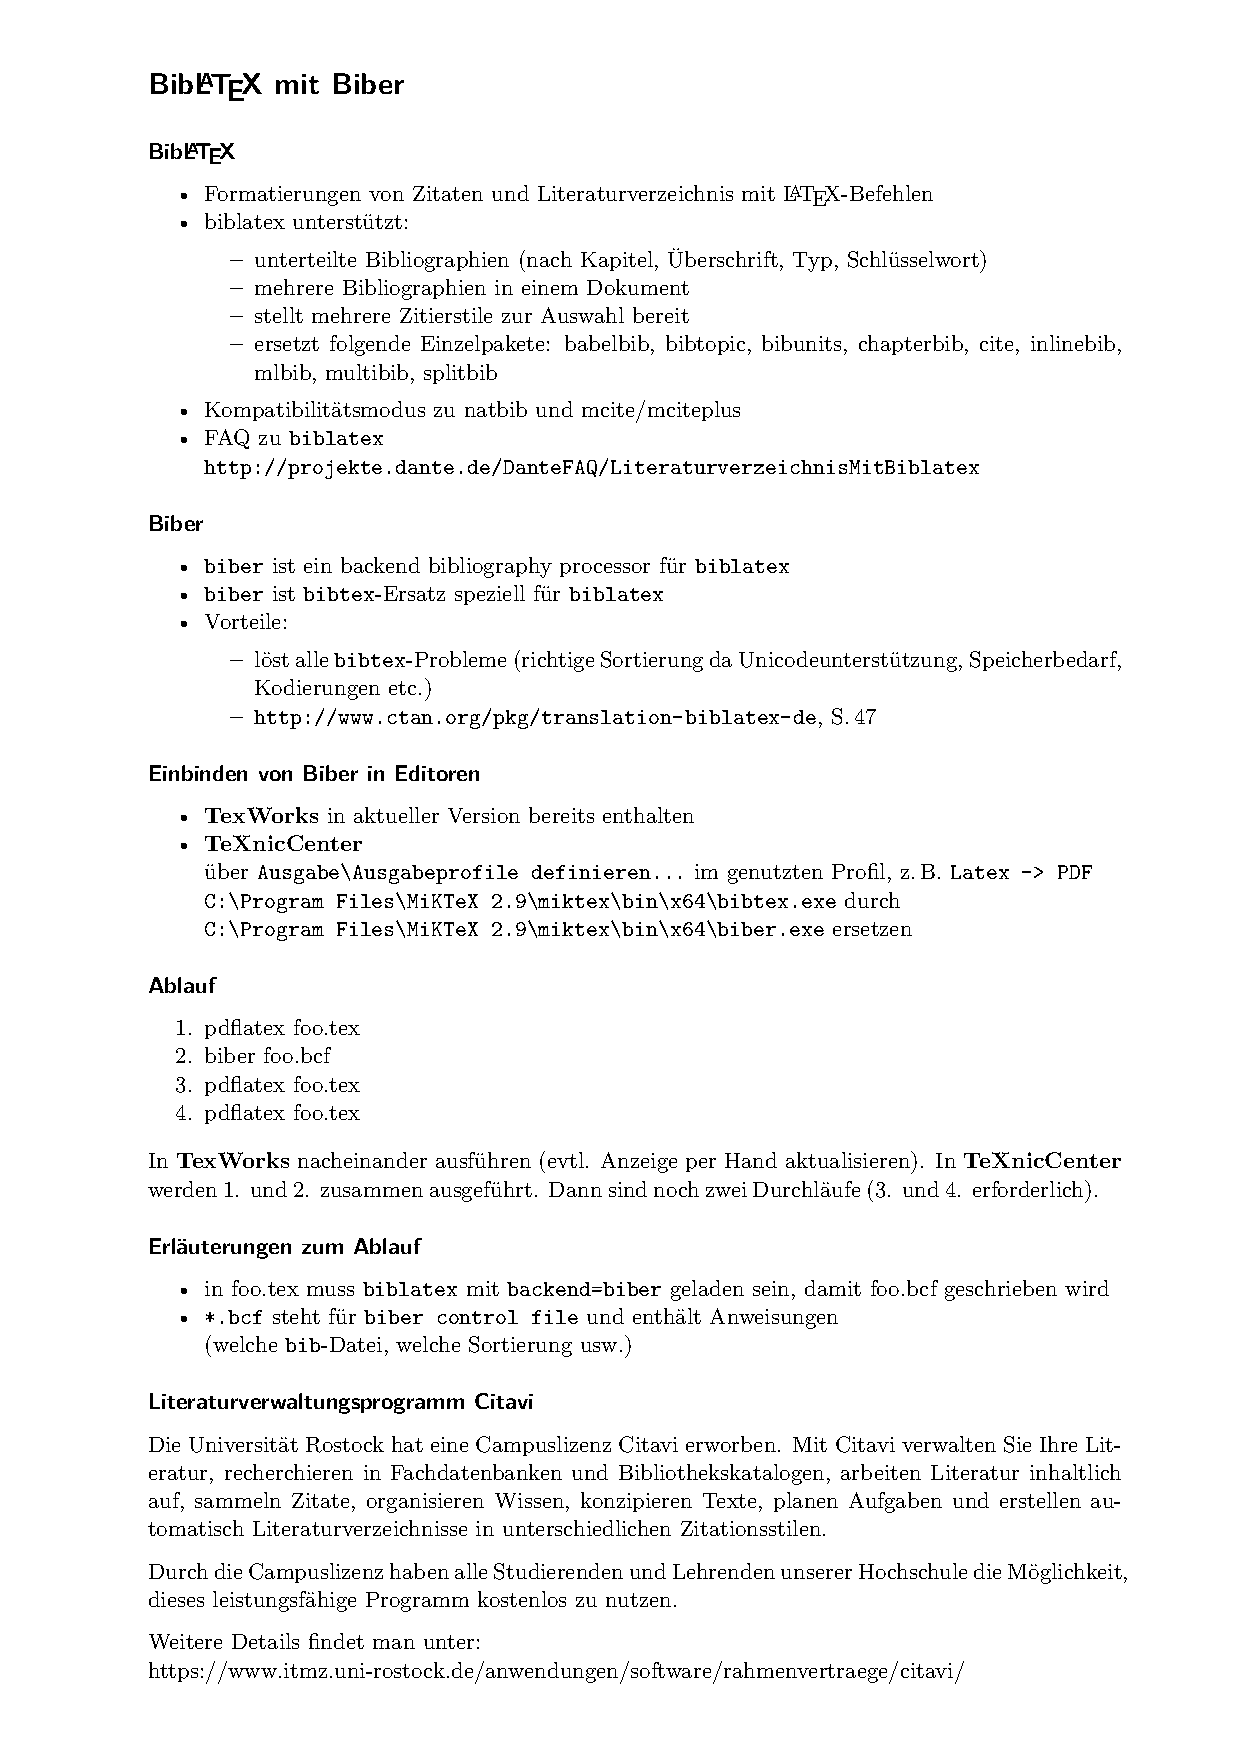
\includepdf[pages={1-2},scale=.9]{AnleitungBibLatexBiber.pdf}


\end{document}
